\documentclass[runningheads]{llncs}

% ---------------------------------------------------------------
% Based on ECCV 2024 template


\usepackage{eccv}

% OPTIONAL: Un-comment the following line for a version which is easier to read
% on small portrait-orientation screens (e.g., mobile phones, or beside other windows)
%\usepackage[mobile]{eccv}


% ---------------------------------------------------------------
% Other packages

% Commonly used abbreviations (\eg, \ie, \etc, \cf, \etal, etc.)
\usepackage{eccvabbrv}

% Include other packages here, before hyperref.
\usepackage{graphicx}
\usepackage{parskip}
\usepackage{booktabs}

% The "axessiblity" package can be found at: https://ctan.org/pkg/axessibility?lang=en
\usepackage[accsupp]{axessibility}  % Improves PDF readability for those with disabilities.


% ---------------------------------------------------------------
% Hyperref package

% It is strongly recommended to use hyperref, especially for the review version.
% Please disable hyperref *only* if you encounter grave issues.
% hyperref with option pagebackref eases the reviewers' job, but should be disabled for the final version.
%
% If you comment hyperref and then uncomment it, you should delete
% main.aux before re-running LaTeX.
% (Or just hit 'q' on the first LaTeX run, let it finish, and you
%  should be clear).

% TODO FINAL: Comment out the following line for the camera-ready version
\usepackage[pagebackref,breaklinks,colorlinks,citecolor=eccvblue]{hyperref}
% TODO FINAL: Un-comment the following line for the camera-ready version
%\usepackage{hyperref}

% Support for ORCID icon
\usepackage{orcidlink}


\begin{document}

% Instructions
% - Please write your reports in \LaTeX~and make them as well-written and presentable as possible, report quality is taken into account in grading.
% - Submit your zipped \LaTeX~files and the PDF to Moodle OR via email to the TAs (\url{ehsan.pajouheshgar@epfl.ch}, \url{martin.everaert@epfl.ch}, \url{raphael.achddou@epfl.ch}).
% - We recommend you the provided template to make things easier for you.
% - You can use Overleaf to collaborate together on the same document and ease compilation of \LaTeX~files.

% - Reports should not exceed 15 pages if you use the provided template format (and equivalent length if you are not using this template). This does not include References and the Appendix. You should be concise and make every sentence and figure convey good information such that everything essential fits the 15 pages. Below is a suggested structure you can follow. You can add more sections if deemed necessary.

% Title & Authors
\title{
    Sillystill: Recreating the Look of Cinestill-800T using Deep Learning
}

\author{Mika Senghaas \quad Annamira O'Toole \quad Pierre Lardet}

\institute{Supervised by Dr. Raphaël Achddou in CS413 at EPFL}

\maketitle
\thispagestyle{empty}

% Abstract
\begin{abstract}

The use of deep learning in stylistic effect generation has seen increasing use over recent years. In this work, we use simple convolutional neural networks to model Cinestill800T film given a digital input. We test the effect of different loss functions, as well as the addition of an input noise channel and the use of random scales of patches during training. We find that a combination of MSE/VGG gives the best colour production, and that some grain can be produced, but it is not of a high quality, and no halation is produced. We contribute our dataset of aligned paired images taken with a film and digital camera for further work.

\end{abstract}

% Report
\section{Introduction}
\label{sec:introduction}

% Maximum 3-4 pages, all external statements must be referenced
% 1. What is the problem in general terms? Why is it important/of interest?
% 2. What other solutions are available? Why are they not good enough? What would we ideally want to have? (-> Narrow down to solutions similar to the last question (i.e. what we ideally want to have), which will be close to our proposition.)
% 3. What are these good similar solutions? How do they work? (some technical insight) What are their limitations?
% 4. What are we proposing? How does it contribute/improve? What do we base our work on, briefly how do we solve?
% 5. What are the assumptions we make? A bit more about the method, what will be presented.

% What is the problem in general terms? Why is it important/of interest?
Film photography is popular among artists and photographers for capturing scenes
in a unique way. They use optical flaws, such as halation and chromatic
aberrations, for aesthetic purposes. Such visual effects are the result of
complex physical processes that are not present in modern digital photography.
Hence, to recreate the visual effects of film in digital images, computational
methods are required. This motivates our work, where we investigate the
feasibility of using a pure deep learning approach to recreate the visual
effects of Cinestill-800T film, an iconic film stock known for its grain
textures, color hues and red halation.

% 2. What other solutions are available? Why are they not good enough? What would we ideally want to have? (-> Narrow down to solutions similar to the last question (i.e. what we ideally want to have), which will be close to our proposition.) What are these good similar solutions? How do they work? (some technical insight) What are their limitations?

Most available solutions involve directly modelling
the physical processes that lead to the visual effects~\cite{film-grain-rendering}. However, the complex
interplay between the camera, film stock, and chemicals during the development
process, means that simplifying assumptions have to be made. In addition, such
models are often computationally expensive and time consuming, especially when applied to
high-resolution images.

Ideally, a digital image could be processed into its film equivalent on the
order of seconds with high fidelity. Deep learning models have shown impressive
results in learning complex mappings, out-performing handcrafted models in many
tasks. One can hope that a deep learning model could learn higher quality
style translations than existing methods, while reducing computational complexity.
However, the problem of recreating film effect has not been directly addressed
by deep learning literature. Related computational photography problems include
camera raw-to-raw mappings, quality enhancement, grayscale colorisation, and
style transfer. As none of these involve direct applicatino to the problem of film
effect generation, we examine the commonly used techniques and how they could be adapted to our task.

% 3. What are we proposing? How does it contribute/improve? What do we base our
% work on, briefly how do we solve? What are the assumptions we make? A bit more
% about the method, what will be presented.
All of this motivates our work, where we investigate the feasibility of using
deep learning to recreate the visual effects of Cinestill-800T film in digital
images. We propose training a U-Net-like model translation network on a
new dataset of paired digital and film images. While we acknowledge
that using direct statistical models for film grain, halation, and color hue may
be effective as a standalone, or in combination with deep learning, we constrain
this work to only explore pure deep learning methods.

Our contributions can be summarised as:

\begin{itemize}
    \item We propose a pure deep learning approach to recreate the visual effects of Cinestill-800T film in digital images.
    \item We present a self-collected dataset of paired digital and film images, which we publicly release to the research community.
    \item We investigate and analyse various techniques that help to improve the creation of visual effects, such as adding noise to the input, training on random-resized crops, or varying the loss function.
\end{itemize}
\section{Literature Review}
\label{sec:literature-review}

% All your statements must be referenced. Any related paper/resource you found should be listed for readers.}

% Go over the entire related literature. Start from general to the most specific related methods.

% For the most related papers, and for all papers/algorithms used in your
% project, you should go more into details and explain what the paper does,
% adding an explanation of their pros and cons and how they compare/relate to
% what you have done in your own work.

Many methods have presented as viable solutions for stylistic effect generation using image to image translation using Deep Learning. Among these, there is a variety of kinds of model architectures and effects produced.

\vspace{5pt}\noindent\textbf{Image Translation.} GANs have seen successful application in generic image translation, such as in Conditional Image-Image Translation \cite{conditionalgan} in which a loss is learned by a discriminator network which is conditioned on the input. This can be generalised to unpaired image data using Cyclic GANs \cite{cyclicgan} where two translation networks are used in either direction, and cyclic consistency is enforced using the loss function.


\noindent\textbf{Super Resolution.} The task of generating a higher resolution image from a lower resolution image has been tackled by deep learning approaches with a variety of pixel-wise and perceptual losses \cite{image-super-resolution-with-deep-networks,accurate-image-super-resolution,resolution-perceptual-losses}. GANs have produced impressive results \cite{gan-photo-realistic-super-resolution, esrgan-super-resolution}, especially in combination with perceptual losses \cite{pulse-gan-perceptual-super-resolution,recovering-texture-super-resolution}. Methods for greater stability during training have been developed \cite{gan-progressive-stability-resolution} and for greater control over which style is produced \cite{gan-style-based-resolution}. 

\noindent A contextual bilateral loss was introduced by \cite{zoom-to-learn} based on RGB and VGG feature patches that builds on the contextual loss proposed by \cite{contextual-loss} by adding a distance weighting. The authors claim that this loss is robust to misalignment in paired datasets. We implemented this loss but found it did not improve our results and do not include it in our final models.

\noindent\textbf{Image Colorisation.} Converting a grayscale image to a color has been attempted by \cite{large-scale-colorisation} using chromaticity maps, and \cite{intrinsic-colorisation} addresses the problem of illuminants by searching the web for reference images. \cite{deep-colorisation} leverages deep learning with separate networks for different kinds of images. This suggests a natural extension of our work would be to condition the digital-film mapping on features such as a luminance histogram.

\noindent\textbf{Raw to Raw Mapping.} \cite{raw-to-raw} maps the raw output of one camera to another using paired auto-encoders. Each auto-encoder is trained on raw outputs from a different camera, and the latent space of the two auto-encoders is mapped using a paired dataset. We implemented this architecture for a digital to film mapping, but it did not produce good initial results so we did not pursue it further.

\noindent\textbf{Style Transfer.} Style transfer, which maps the style of one image to the content of another, has seen success using CNNs which are trained to minimize a content and style loss. This has been applied to paintings \cite{image-style-transfer, scaling-painting-style-transfer} and to photorealistic images \cite{deep-photo-style-transfer}. These methods require an expensive optimization for every image. Instead, \cite{resolution-perceptual-losses} uses perceptual losses based on VGG features to train a feed forward model and \cite{arbitrary-style-transfer} extends this to arbitrary styles using adaptive instance normalization. \cite{dslr-quality} attempts to convert the style of phone images to DSLR quality using a composite loss including functions for colour, texture and content. We follow a similar approach in our work, using perceptual features produced by VGG-19 \cite{vgg} as part of our loss to train a feed forward CNN for style transfer.


% ---------------------------------------------------------
% \noindent\textbf{Super Resolution.} Super-resolution involves generating a higher resolution image from a lower resolution one. Existing approaches either train on paired datasets of low resolution and high resolution images of the same scene, or a dataset of high resolution images with their downsampled low-quality versions.

% Generally, CNN-based methods for super resolution involve downsampling a high-resolution before feeding it through a CNN which involves both convolutional layers and upsampling layers. Often loss is defined based on the L1 or L2 norm between the original high resolution image and the upsampled output image. Training with loss based on average distance metrics between high quality and low quality images tends to produce a blurring affect, as noted in \cite{photo-realistic-super-resolution} and \cite{dslr-quality}. Success of a super resolution model is often measured by the Peak Single to Noise Ratio (PSNR), which is directly optimized by simple MSE losses. In \cite{dslr-quality} different loss functions are employed which combine analytical content and color losses with an adversarially learned texture loss. 

% To avoid the challenge of producing perceptually good results with CNNs, approaches such as \cite{pulse-super-resolution} and \cite{photo-realistic-super-resolution} use Generative Adversarial Networks (GANs). In this case, a generative model is trained to produce high resolution images based on low-quality images that are able to fool discriminator trained to distinguish super-resolved images from real images.

% Implementation
\section{Implementation}
\label{sec:implementation}

% Guidelines:
% - Justify as much as possible all your design choices. Make clear all the details needed to reproduce your results.}
% - Divide your project into different sections, and explain each one here.
% - Add as many illustrations and graphs/charts as possible to make sure your ideas are conveyed clearly. The goal is to make sure what you have done is clearly explained to be graded fairly.

To recreate the look of Cinestill-800T we aim to train a deep image-to-image
translation network on a paired digital-film dataset. This requires a dataset of
digital images and their corresponding film images, a suitable model
architecture, and loss functions capable of capturing the appearance of film.

\subsection{Data Collection and Preprocessing}
\label{subsec:data}
\label{subsubsec:data-collection}

% Motivation
While unpaired digital or film datasets are abundant, our method requires paired digital-film images. This means that the exact same scene has to be captured with both a digital and a film camera to allow the model to learn the differences in appearance between the two media. Images should be aligned, as our model should only transfer style and not learn move contents of the image around, and diverse in order to capture Cinestill-800T's baheviour in a variety of scenes and lighting conditions. As no such dataset was available, we collected our own.

% Dataset collection
\textbf{Data Collection.} To ensure aligned images, we take inspiration from the setup proposed in~\cite{dslr-quality} and capture images with two cameras, a Sony Alpha 7 digital camera and a Nikon F3 film camera. Photos were taken by keeping the same tripod setup for both cameras for each image. Camera settings like aperture, ISO and shutter speed were kept constant across both cameras as best as possible (Table~\ref{tab:cameras}). We only captured static scenes to limit changes in the scene between shots. To create a diverse dataset, images were taken both indoors and outdoors, in different weather conditions, with different light and containing different subjects. Specific emphasis was put on ensuring that all special visual effects (halation, grain and colours) were well-represented in the dataset. The final raw dataset consists of 41 image pairs. Some examples are presented in Figure~\ref{fig:raw-dataset}. 

\begin{table}
    \centering
    \caption{Camera Setup.}
    \begin{tabular}{lccccc}
        \toprule
        \textbf{Camera} & \textbf{Resolution} & \textbf{Lens} & \textbf{Aperture} & \textbf{ISO} & \textbf{Shutter} \\
        \midrule
        Sony Alpha 7 (Digital) & 24 MP & 40mm & F8 & 100 & Auto \\
        Nikon F3 (Film) & 12 MP & 55mm & F8 & 100 & Auto\\
        \bottomrule
    \end{tabular}
    \label{tab:cameras}
\end{table}

% TODO: Maybe introduce notation to refer to dataset
% $D_{\text{raw}}=\{(I^F_n, I^D_n)\}_n^{41}$
% TODO: Maybe talk about resolution of digital/ film images
% TODO: Maybe talk about processing to JPEG

\begin{figure}
    \begin{subfigure}[t]{.19\textwidth}
      \centering
      \includegraphics[width=\linewidth]{figures/digital1.jpeg}
    \end{subfigure}
    \hfill
    \begin{subfigure}[t]{.19\textwidth}
      \centering
      \includegraphics[width=\linewidth]{figures/digital2.jpeg}
    \end{subfigure}
    \hfill
    \begin{subfigure}[t]{.19\textwidth}
      \centering
      \includegraphics[width=\linewidth]{figures/digital3.jpeg}
    \end{subfigure}
    \hfill
    \begin{subfigure}[t]{.19\textwidth}
      \centering
      \includegraphics[width=\linewidth]{figures/digital4.jpeg}
    \end{subfigure}
    \begin{subfigure}[t]{.19\textwidth}
      \centering
      \includegraphics[width=\linewidth]{figures/digital5.jpeg}
    \end{subfigure}
  
    \medskip

    \begin{subfigure}[t]{.19\textwidth}
      \centering
      \includegraphics[width=\linewidth]{figures/film1.jpeg}
    \end{subfigure}
    \hfill
    \begin{subfigure}[t]{.19\textwidth}
      \centering
      \includegraphics[width=\linewidth]{figures/film2.jpeg}
    \end{subfigure}
    \hfill
    \begin{subfigure}[t]{.19\textwidth}
      \centering
      \includegraphics[width=\linewidth]{figures/film3.jpeg}
    \end{subfigure}
    \hfill
    \begin{subfigure}[t]{.19\textwidth}
      \centering
      \includegraphics[width=\linewidth]{figures/film4.jpeg}
    \end{subfigure}
    \begin{subfigure}[t]{.19\textwidth}
      \centering
      \includegraphics[width=\linewidth]{figures/film5.jpeg}
    \end{subfigure}
  
    \caption{\textbf{Raw Paired Image Dataset.} Examples of raw image pairs from the dataset. A column shows a single scene captured with a digital camera (top) and a film camera (bottom). The images show a wide range of scenes and visual effects.}
    \label{fig:raw-dataset}
\end{figure}



\subsubsection*{Data Preprocessing}
\label{subsubsec:preprocessing}

Inevitably, raw image pairs are not perfectly aligned. To address this
issue, we first spatially align the images using keypoint alignment. We follow a standard processing pipeline using openly available implementations of common feature detection, matching and perspective transformation algorithms from the OpenCV library~\cite{opencv}. For all image pairs we first detect keypoints and extract descriptors using ORB~\cite{orb}, match them using FLANN~\cite{flann}, and estimate a homography transformation matrix using the \href{https://www.mathworks.com/discovery/ransac.html}{RANSAC} algorithm.

% Luminance Alignment
To ensure that our model does not learn systematic brightness adjustments, we also align the luminance of each image pair. We align the luminance of the film image to the digital image as our model receives digital as input at inference time. The luminance alignment is performed using histogram matching on the luminance channel in CIELAB space before converting back to RGB.

% \begin{enumerate}
%     \item \textbf{Convert to CIELAB} We convert both the digital and film images to the CIELAB colour space, where the $L$-channel corresponds to luminance.
%     \item \textbf{Histogram Matching} We then match the luminance histogram of the film image to the digital image. This is done by computing and interpolating the cumulative distribution function (CDF) of the luminance channel of both images.
%     \item \textbf{Convert back to RGB} Finally, we convert the film image back to the RGB colour space.
% \end{enumerate}

An example of the results of these two steps can be seen in Figure~\ref{fig:data-preprocessing}. After the
preprocessing steps we are left with 38 processed image pairs. We publicly
release both the raw and processed dataset to facilitate further work.

% \begin{enumerate}
%     \item \textbf{Keypoint Detection} We use the ORB~\cite{orb} (Oriented FAST and Rotated BRIEF) feature detection algorithm to detect keypoints and extract descriptors from both images.
%     \item \textbf{Keypoint Matching} We then use the FLANN~\cite{flann} (Fast Library for Approximate Nearest Neighbors) algorithm to match the keypoints between the images. We apply the Lowe's ratio test to filter out matches that are likely to be incorrect.
%     \item \textbf{Homography Estimation} Finally, we estimate a homography matrix using a subset of the matched keypoints using the RANSAC algorithm~\cite{ransac}. The matrix defines a perspective transformation which we apply to the digital image to align it with the film image.
% \end{enumerate}

% Could go into more detail about the maths behind the algorithms and algorithms' parameters used in our experiments. Absolutely Not. 

% Could mention that we tried other keypoint detection algorithms: Absolutely Not.
% We also experimented with other keypoint detection algorithms, such as SIFT (Scale-Invariant Feature Transform)~\cite{sift} and SURF (Speeded-Up Robust Features)~\cite{surf}, and simple brute-force feature matching algorithms, but found that the above pipeline provided accurate results and did not require a patent license.



\begin{figure}
    % \begin{subfigure}[t]{.24\textwidth}
    %   \centering
    %   \includegraphics[width=\linewidth]{figures/raw-film.jpeg}
    %   \caption{Raw Film Image}
    % \end{subfigure}
    % \hfill
    % \begin{subfigure}[t]{.24\textwidth}
    %   \centering
    %   \includegraphics[width=\linewidth]{figures/processed-film.jpeg}
    %   \caption{Processed Film Image}
    % \end{subfigure}
    % \hfill
    % \begin{subfigure}[t]{.24\textwidth}
    %   \centering
    %   \includegraphics[width=\linewidth]{figures/raw-digital.jpeg}
    %   \caption{Raw Digital Image}
    % \end{subfigure}
    % \hfill
    % \begin{subfigure}[t]{.24\textwidth}
    %   \centering
    %   \includegraphics[width=\linewidth]{figures/processed-digital.jpeg}
    %   \caption{Processed Digital Image}
    % \end{subfigure}


    \begin{subfigure}[b]{0.49\textwidth}
      \centering
      \includegraphics[width=0.49\textwidth]{figures/raw-film.jpeg}
      \includegraphics[width=0.49\textwidth]{figures/processed-film.jpeg}
      \captionsetup{justification=centering}
      \caption{Film: Raw (left) vs. Processed (right).} 
  \end{subfigure}
  \hfill
  \begin{subfigure}[b]{0.49\textwidth}
      \centering
      \includegraphics[width=0.49\textwidth]{figures/raw-digital.jpeg}
      \includegraphics[width=0.49\textwidth]{figures/raw-film}
      \captionsetup{justification=centering}
      \caption{Digital: Raw (left) vs. Processed (right).}
  \end{subfigure}

    \caption{\textbf{Dataset Preprocessing.} Example of a raw and processed image pair. We can see the luminance alignment in the film image (a) and the spatial alignment in the digital image (b).}
    \label{fig:data-preprocessing}
\end{figure}

% Maybe talk about data augmentation (horizontal/ vertical flips, brightness adjustment and blur)
% We didn't do this for our final runs, so no.
\subsection{Model}
\label{subsec:model}

Our image style translation network is based on the U-Net
architecture~\cite{unet}. U-Net is a type of convolutional neural network (CNN)
originally introduced for image segmentation tasks in 2015. CNNs have been
successfully adapted for various image-to-image translation tasks and similar models are used as the
building block of many modern model families, such as auto-encoders \cite{raw-to-raw} and GANs \cite{perceptual-losses-style-transfer}. The network features a U-shaped architecture, composed of an encoder and a decoder. The encoder
resembles a conventional convolutional network, involving repeated convolutions
followed by a non-linear activation functions and pooling operations. The decoder integrates both feature and spatial information using up-convolutions and high-resolution features via skip connections.

% Motivation for using U-Net
We selected UNet as it is a relatively simple model family, allowing us to focus on
the specifics of our problem rather than the intricacies of the model. Despite its simplicity, similar models such as CNNs with residual connections have been shown to be effective for image-to-image translation, such as in \cite{dslr-quality}. As it is fully convolutional, it can be applied to images of arbitrary size.
\footnote{So long as the input dimensions are divisible by $2^L$, where $L$ is
the number of layers in the encoder}
% This allows us to experiment
% with training on smaller image patches and applying the network to larger images
% at test time with no architectural changes or pre-processing steps.

% TODO: Maybe add some more citations on related work using U-Net

% TODO: Add figure for U-Net architecture

% Detailed model architecture
For our experiments we follow related work \cite{unet,dslr-quality,raw-to-raw}
to set sensible hyperparameters for our model. Our image style translation
network is fully convolutional, with a three-layer encoder and decoder. The encoder consists of three convolutional blocks with 64, 128, and 256 filters, respectively. Each block consists of two convolutional layers with 3×3 kernels and zero padding, interleaved with ReLu activation functions.
In between each of the convolutional blocks, we downsample the spatial dimension
of the feature maps by a factor of two using a 2×2 max-pooling operation. The
decoder performs the reverse operation by upsampling the spatial
dimension. It decreases the number of filters from 256 to 128, 64, and finally
to 3. Upsampling is performed via a 2×2 transposed convolution. After
upsampling, we concatenate the feature maps from the corresponding layer in the
encoder before applying a convolutional block. After the final layer,
the model outputs a three-channel image, corresponding to the RGB channels of
the transformed image. Thus, the overall translation network $F_{\theta}$
is an image-to-image model, that takes an image $I$ as input and outputs a
transformed image $F_{\theta}(I)$ of the same dimensions. 
% Both input and output are three-dimensional tensors of size $3 \times H \times W$, where $3$ correspond to the RGB channels and $H$ and $W$ are the height and width of the image, respectively. The total number of parameters in the model is approximately 1.9M, corresponding to a memory footprint of around 7.6MB.

% TODO: Maybe mention that we don't employ normalisation/ dropout layers

% \begin{table}{ccc}
%     \centering
%     \caption{
%         \textbf{Model architectures.} The table shows the base model architecture that is used for all experiments, unless otherwise specified.
%     }
%     \label{tab:model}
%     \begin{tabular}{ccc}
%         \toprule
%         \# Input Channels & \# Hidden Channels & Convolution & Pooling & Non-Linearity \\
%         3 & 64, 128, 256 & 3x3 (1) & 2x2 Max & ReLU \\
%         \midrule
%         \bottomrule
% \end{table}
\subsection{Loss Functions}
\label{subsec:loss-functions}

We propose a list of loss functions that can be combined, each targeting different effects.

\textbf{MSE/MAE.} Both the mean squared error (MSE, Eq.~\ref{eq:mse}) and mean absolute error (MAE, Eq.~\ref{eq:mae}) are common pixel-to-pixel loss functions, that are popular in image reconstruction tasks. They measure the average squared or absolute difference between the predicted and ground truth images pixels, respectively. For two images, $X, Y \in \mathbb{R}^{3 \times H \times W}$, the MSE and MAE losses are defined as:
\begin{multicols}{2}
\begin{equation}
    \mathcal{L}_\text{MSE}(X, Y) = \frac{1}{n} \sum_{i=1}^{n} (X_i, Y_i)^2
    \label{eq:mse}
\end{equation}

\begin{equation}
    \mathcal{L}_\text{MAE}(X, Y) = \frac{1}{n} \sum_{i=1}^{n} |X_i - Y_i|
    \label{eq:mae}
\end{equation}
\end{multicols}

where $i$ indexes the pixels of the images. We hypothesise that
such loss functions are useful in preserving the overall structure and color of the image,
but are not sufficient to capture higher-level visual effects such as grain and
halation.

\textbf{VGG Loss.} VGG loss computes the MSE (Eq.~\ref{eq:mse}) between the feature representations of the predicted and ground truth images when passed through a pre-trained VGG-19~\cite{vgg} convolutional network. Letting $\varphi_k(I)$ denote the feature maps of the $k$-th layer of the VGG network, and the sets $K$ and $\lambda$ denote the layers of interest \footnote{We use conv1\_2, conv2\_2, conv3\_2 with weights 0.4, 0.4 and 0.2 respectively.} and their weights in the loss function respectively, the VGG loss is defined as:

\begin{equation}
   \mathcal{L}_\text{VGG}(X, Y) = \sum_{k \in K} \lambda_k \mathcal{L}_\text{MSE}(\varphi_k(X), \varphi_k(Y)).
    \label{eq:vgg}
\end{equation}

Intuitively, the VGG loss encourages the model to generate images that are similar to the ground truth images in terms of their high-level semantics such 
as edges, textures and patterns.

\textbf{Color Loss.} Inspired by~\cite{dslr-quality}, we consider an alternative to the MSE loss, which we refer to as the color loss. The color loss computes the MSE between two images, $X_b$ an $Y_b$, where $X_b$ and $Y_b$ are blurred versions of the predicted and ground truth images respectively. Blurring is done using a Gaussian filter with a kernel size of 7 and \(\sigma=3\). We can write:

\begin{equation}
    \mathcal{L}_\text{Color}(X, Y) = \mathcal{L}_\text{MSE}(X_b, Y_b).
    \label{eq:color}
\end{equation}

As the authors of the original paper argue, the main idea behind the loss is to evaluate the brightness, contrast and major colours of the image while ignoring fine-grained texture and content comparison. Crucially, the color loss, unlike MSE or MAE, is more robust to small pixel shifts which are present in our training data.

\textbf{Relative Total Variational Loss (TV-Rel).} Traditionally, the \href{https://lightning.ai/docs/torchmetrics/stable/image/total_variation.html}{total variational} loss is used to encourage image smoothness and reduce noise by minimising the sum of the absolute differences between shifted pixel values. In our case, we aim to create grain, which can be seen as a form of noise. To this end, we propose the relative total variational loss defined as the absolute difference between the total variation of the predicted and ground
truth images. 

\begin{equation}
    \mathcal{L}_\text{TV-Rel} = |TV(X) - TV(Y)| 
    \label{eq:tv-rel}
  \end{equation}

This loss encourages the model to generate images with a similar
amount of noise to the ground truth film images.

\textbf{Combination of Losses.} We combine the individual loss functions to form the final loss function using a weighted sum. For a set of loss functions $\mathcal{L}$ and corresponding weights $\beta$ \footnote{We simply use equal weights in all experiments with $\beta_i = 1$ for all $i$}, the final loss function is defined as

\begin{equation}
    \mathcal{L}(X, Y) = \sum_{i} \beta_i \mathcal{L}_i(X, Y).
    \label{eq:combined-loss}
\end{equation}

Some combinations of loss functions are more effective than others, and we will experiment with different combinations, as outlined in Section \ref{sec:results}.

% \textbf{CoBi Loss.} Introduced by \cite{zoom-to-learn}, Contextual Bilateral Loss (CoBi Loss) is inspired by the bilateral filter \cite{bilateral-filter} which preserves-edges while reducing noise. The motivation for its design is to judge image feature similarity even when an image pair is misaligned. CoBi Loss combines spatial pixel coordinates and pixel-level RGB information for a nearest neighbor search on image features. 
% 
% \begin{definition}
%   \textbf{CoBi Loss}
% \begin{equation}
%   \text{CoBi}(P, Q) = \frac{1}{N}\Sigma_{i,j}\min_{j=1,...M} (D_{p_i,q_i} + \omega_s D'_{p_i, q_i})
% \end{equation}
% \end{definition}
% 
% Where $P$ and $Q$ are the predicted and ground truth images with $N$ and $M$ feature points respectively. $\omega_s$ is a hyperparameter that controls the influence of the spatial awareness for nearest neighbor search. $D_{p_i,q_i}$ and $D'_{p_i,q_i}$ are distance measurements between feature points of the predicted and ground truth images. 

% TODO: Talk about combination of losses. 
\subsection{Experiments}
\label{subsec:experiments}

The training procedure is illustrated in Figure~\ref{fig:training-overview}. We train our model on a dataset of paired digital-film images. As our image dataset is relatively small, we use a patched training approach, where we randomly sample patches of size $256 \times 256$ from the images before feeding them into the model. We train our model on 400 patches per image in the dataset using the Adam optimizer with a learning rate of $1e-3$ and a batch size of 1. Our experiments are divided into two parts: single-image experiments and full dataset experiments.

\begin{figure}
  \centering
  \includegraphics[width=0.9\textwidth]{figures/training-overview.png}
  \caption{\textbf{Training Overview.} We train our model on paired digital-film images.}
  \label{fig:training-overview}
\end{figure}

% Single image experiments
For our single-image experiments, we handpicked an image from our dataset that contains a white wall with a light source. It was chosen for the clear blue tint of the film effect and the clearly perceptible grain on the uniform background. For these experiments, we train and evaluate the model on the same image. We first investigate how each loss produces the desired colour effect to gain a better understanding of the interplay between the loss functions and what the model learns.

% Full dataset experiments
For the most promising candidates from the single-image experiments, we then
move on to training on the full dataset. The full dataset is split into a
training, validation and test set using a 70-20-10 split ratio, but final evaluation is done on the full dataset.

% Adding noise channel and resizing
We also investigate whether adding noise as a 4th input channel to the model improves the its ability to learn the desired visual effects for both single image and full dataset experiments. This is done by concatenating a random uniform noise \footnote{We tried using other forms of noise such as Guassian noise but found that this made little difference.} channel to the input images.  Furthermore, we observed that patched training is very stochastic as each patch only captures a very small portion of the original image and can be very different from the rest of the image. To contain more information in each patch we also experiment applying a resized crop where we first crop the image to a larger patch and then resize to the desired input size. This way we can ensure that each patch contains more information from the original image.


\subsection{Evaluation}
\label{subsec:evaluation}

% Qualitative assessment: Visual comparison of results (patches during training/
% evaluation + inference on downsampled images on full dataset)
To evaluate the generated film images, we conduct both qualitative and
quantitative assessments. For quantitative evaluation, we use four image quality and image similarity metrics. We include a reference baseline comparison which is calculated using the original digital image as the prediction.

We use two standard algorithmic metrics, \textbf{Peak Signal-to-Noise Ratio (PSNR)}, which measures the ratio of the maximum possible signal power to the power of corrupting noise, and \textbf{Structural Similarity Index (SSIM)}, which compares structural, luminance, and contrast elements between an original and a reconstructed image in a range from -1 to 1. We also use two learned distance metrics, \textbf{Learned Perceptual Image Patch Similarity (LPIPS)} \cite{LPIPS} and \textbf{PieApp} \cite{PieAPP}, where lower indicates higher similarity, which are trained on human-annotated data to align with human perception of image quality.

% \textbf{Peak Signal-to-Noise Ratio (PSNR)} assesses the quality of a
% reconstructed image compared to its original by calculating the ratio of the
% maximum possible signal power to the power of corrupting noise. High PSNR values
% indicate better image quality, implying less noise corruption. However, PSNR
% can be sensitive to small pixel
% variations. \textbf{Structural Similarity Index (SSIM)} measures image quality by comparing
% structural, luminance, and contrast elements between an original and a
% reconstructed image. SSIM values range between -1 and 1, where 1 signifies
% perfect similarity. It aligns more closely with human visual perception compared
% to PSNR and is less sensitive to minor pixel changes, making it more reflective
% of perceived image quality.

% \textbf{Learned Perceptual Image Patch Similarity (LPIPS)}~\cite{LPIPS} is a
% learned distance metric based on VGG features, capturing perceptual image quality based
% on human-annotated data.Lower LPIPS values indicate higher similarity between the
% images.

% \textbf{PieApp}, like LPIPS, is a learned metric designed to align with human
% perception. It defines a perceptual error score between a distorted image and
% its reference, representing human-perceived distortion magnitude. Lower PieApp
% scores indicate higher similarity between images.



% More details from Annamira:
% \textbf{Peak Signal-to-Noise Ratio (PSNR).} The Peak Signal-to-Noise Ratio (PSNR) is a frequently used pixel-based metric to evaluate the quality of a reconstructed image. It measures the ratio between the maximum possible power of a signal and the power of the noise that affects the fidelity of its representation. If the PSNR value is high, the quality of the image is high, as it implies a low level of corrupting noise.
% 
% We denote the Mean Squared Error (MSE) between an original $m$-by-$n$ pixel image $I$ and the reconstructed image $J$, as $\text{MSE}(I, J)$. The PSNR is then defined using MSE as:
% 
% \begin{equation}
%     \text{PSNR}(I, J) = 10 \cdot \log_{10} \left( \frac{{\text{MAX}_I}^2}{\text{MSE}(I, J)} \right)
%     \label{eq:psnr}
% \end{equation}
% 
% where $\text{MAX}_I$ is the maximum possible pixel value of the image. The PSNR is usually expressed in decibels (dB).
% 
% As an image similarity metric, PSNR has several limitations. It does not take into account the human visual system's perception of image quality, and it is sensitive to small changes in pixel values. This means that small changes in the image can lead to large changes in the PSNR value. For this reason, PSNR is often used in combination with other image quality metrics to provide a more comprehensive evaluation of image quality.
% 
% We use PSNR to compute the pixel-wise similarity between the ground truth film image and the predicted film images. Given PSNR's sensitivity to noise patterns in the image, we expect PSNR to report high values when the model is able to accurately predict noise patterns in the film image. However, the exact placement of the noise pattern is likely to drastically effect the pixel-by-pixel MSE computation for PSNR, and therefore the PSNR value may not be a useful judgement of similarity between real and generated film.
% 
% Therefore, we expect PSNR to judge predictions most positively when we use MSE loss, as opposed to other loss functions.
% 
% \textbf{Structural Similarity Index (SSIM).} The Structural Similarity Index (SSIM) is a pixel-based metric for measuring the similarity between two images. It is based on the assumption that the human visual system is highly sensitive to structural information in images, and that the perceived quality of an image is determined by the similarity of its structure to the structure of a reference image.
% 
% SSIM is designed to capture three aspects of image quality: luminance, contrast, and structure. As these aspects are not judgements of color accuratecy, SSIM is often computed based on the luminance channel of the image, or individually over the red, green, and blue channels and then combined to create a final signal. In our implementation
% 
% The SSIM index is defined as:
% 
% \begin{equation}
%     \text{SSIM}(I, J) = \frac{(2\mu_I\mu_J + C_1)(2\sigma_{IJ} + C_2)}{(\mu_I^2 + \mu_J^2 + C_1)(\sigma_I^2 + \sigma_J^2 + C_2)}
%     \label{eq:ssim}
% \end{equation}
% 
% where $\mu_I$ and $\mu_J$ are the average pixel values of images $I$ and $J$, $\sigma_I^2$ and $\sigma_J^2$ are the variances of images $I$ and $J$, $\sigma_{IJ}$ is the covariance of images $I$ and $J$, and $C_1$ and $C_2$ are constants to stabilise the any division with weak a denominator. The SSIM index ranges from -1 to 1, where 1 indicates perfect similarity between the images.
% 
% Given SSIM's sensitivity to structural information in the image, we expect SSIM to report high values when the model is able to accurately predict the structure and/or grain of the film image, but not be sensitive to the accuracy of the color hue, saturation, or grain. We expect SSIM to be a more robust metric than PSNR, closer in agreement with human perception, as it is less sensitive to small changes in pixel values and more closely aligns with the human visual system's perception of image quality.
% 
% % - LPIPS
% 
% \subsubsection{Learned Perceptual Image Patch Similarity (LPIPS)}
% 
% Proposed in \cite{LPIPS}, the Learned Perceptual Image Patch Similarity (LPIPS) metric is a learned metric based on VGG features. As features of the VGG network trained on ImageNet classification are useful as training loss for image synthesis, it follows that these features should capture some kind of perceptual quality of images. The LPIPS metric computes the distance between two images based on the distance between their VGG features. 
 
% LPIPS is trained on a human-annotated dataset of images along with several distorted copies of each imgage. Humans were asked to choose the most similar image to the original image from the distorted images. The LPIPS metric is then trained to predict the human choice on this dataset.
% 
% We expect LPIPS to be a more robust metric than PSNR and SSIM, as it is trained on human-annotated data and should more closely align with a human's subjective opinion of image quality.  
% 
% % - PieAPP
% 
% \subsubsection{Perceptual Image-Error Assessment through Pairwise Preference (PieApp)}
% 
% Similar to LPIPS, the Perceptual Image-Error Assessment through Pairwise Preference (PieApp) metric is a learned metric trained on a large-scale dataset labeled with the probability that humans will prefered one image over another \cite{PieAPP}. PieApp trains a pairwise-learning framework to predict the preference of one distorted image over the other, similar to LPIPS. 
% 
% PieApp defines a \textit{perceptual error} score between a distorted image and its reference which represents the magnitude of human-perceived distortion. The key observation is that PieApp's trained network can predict a human's perception of error without ever being trained on explicit human perceptual-error labels, but rather only on human preference labels.
% 
% Like LPIPS, we expect PieApp to be a more robust metric than PSNR and SSIM, as it is trained on human-annotated data. We expect both PieApp and LPIPS to align most closely with a human's subjective opinion of image quality.


\section{Results}
\label{sec:results}

% Guidelines: 
% - Emphasis on clarity and reporting results neatly in an organized readable way.
% - Conclude with a summary of all meaningful results you were able to obtain during your project. If possible, all results are benchmarked or compared to state-of-the-art results.
% - Your results should be accompanied by an analysis showing your understanding of why some approach outperforms another, and in what sense/cases it does so.
% - And lastly, discuss the limitations you faced (not implementation problems, but limitations to the project itself), and what you think can be improved.

% We perform experiments in 3 dimensions: loss function, the presence of a noise channel, and whether or not to resize our cropped patches during training.  First, we obtain results for a single image from which we select the best performing configurations to evaluate on the full dataset. 

% Our analysis and evaluation focuses on two effects: colour and grain. We perform quantitative evalution using the previously mentioned metrics: PSNR, SSIM, LPIPS and PieAPP. However, much of our evaluation is based on qualitative assessment, as the perceptual quality of the film effects is the most important aspect of our results. We also include a reference baseline comparison which is calculated using the original digital image as the prediction, or equivalently a model that performs the identity mapping. 

A comprehensive list of all results and experiments can be found in the Appendix Section \ref{sec:all-results}.

\subsection{Single Image Results}

% We selected an image from our dataset that contains a white wall with a light source. It was chosen for the clear blue tint of the film effect and the visually perceptible grain on the uniform background.  We first evaluate how each loss produces the desired colour effect. 

Table \ref{tab:single-image-losses} shows each loss configuration with and without an added noise channel and without resizing. We find that the best performing loss configuration is a combined loss of Color/VGG/TV-Rel, which produces the best SSIM score without noise, and the best PieAPP score in either setting. Notably, the combined losses all perform well, as they account for both the colour and grain effects. The colour-focused losses (MAE, MSE and Colour) all perform well alone, whereas all feature-based losses (VGG and TV-Rel) almost always perform below the baseline. Interestingly, LPIPS scores are inconsistent with the other metrics with the best performing configuration as the baseline and TV-Rel alone with and without noise respectively. This is contrary to what we would be expect as can be seen in a sample of results in Figure \ref{fig:single-image-samples}.

\begin{figure}
    \begin{subfigure}[t]{.19\textwidth}
        \centering
        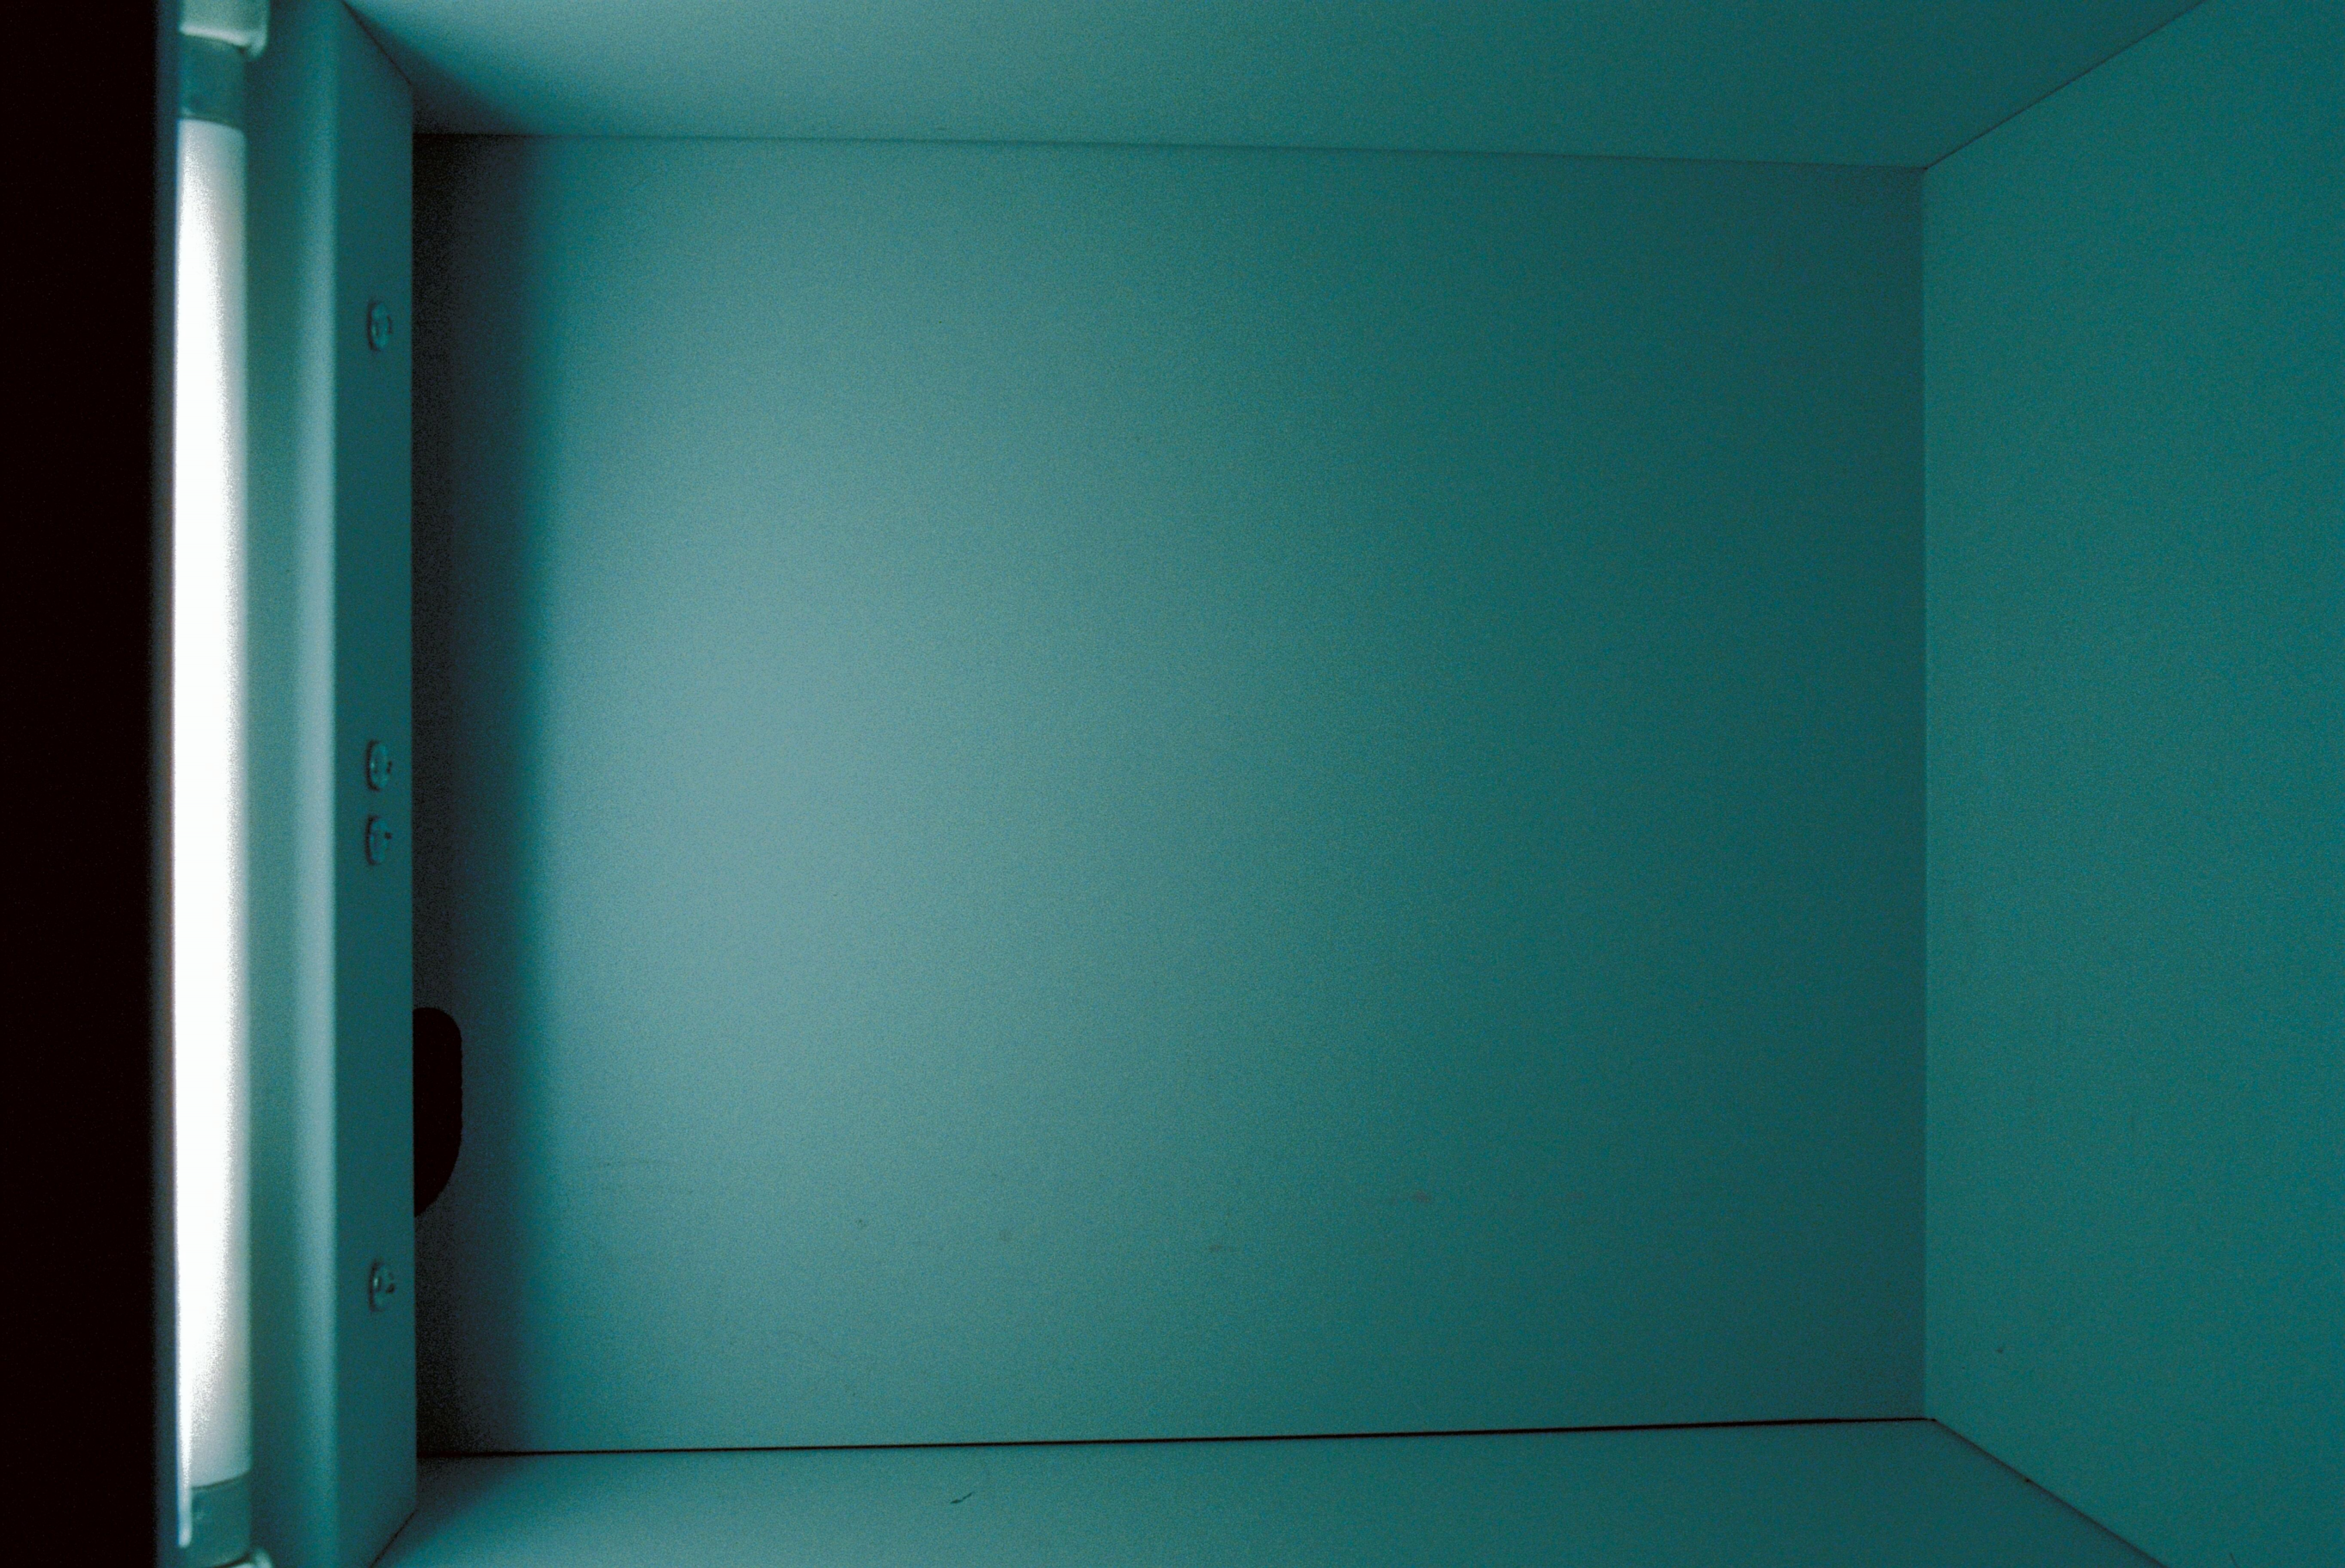
\includegraphics[width=\linewidth]{figures/film-single.png}
        \caption{Film \\ Ground truth}
      \end{subfigure}
    \hfill
    \begin{subfigure}[t]{.19\textwidth}
        \centering
        \includegraphics[width=\linewidth]{figures/mse-vgg-no-noise-resize-single.png}
        \caption{MSE/VGG \\ no noise, resize \\ LPIPS: 0.35 \\ SSIM: \textbf{0.71}}
      \end{subfigure}
    \hfill
    \begin{subfigure}[t]{.19\textwidth}
        \centering
        \includegraphics[width=\linewidth]{figures/mse-no-noise-no-resize-single.png}
        \caption{MSE \\ no noise, no resize \\ LPIPS: 0.47 \\ SSIM: 0.67}
      \end{subfigure}
    \hfill
    \begin{subfigure}[t]{.19\textwidth}
      \centering
      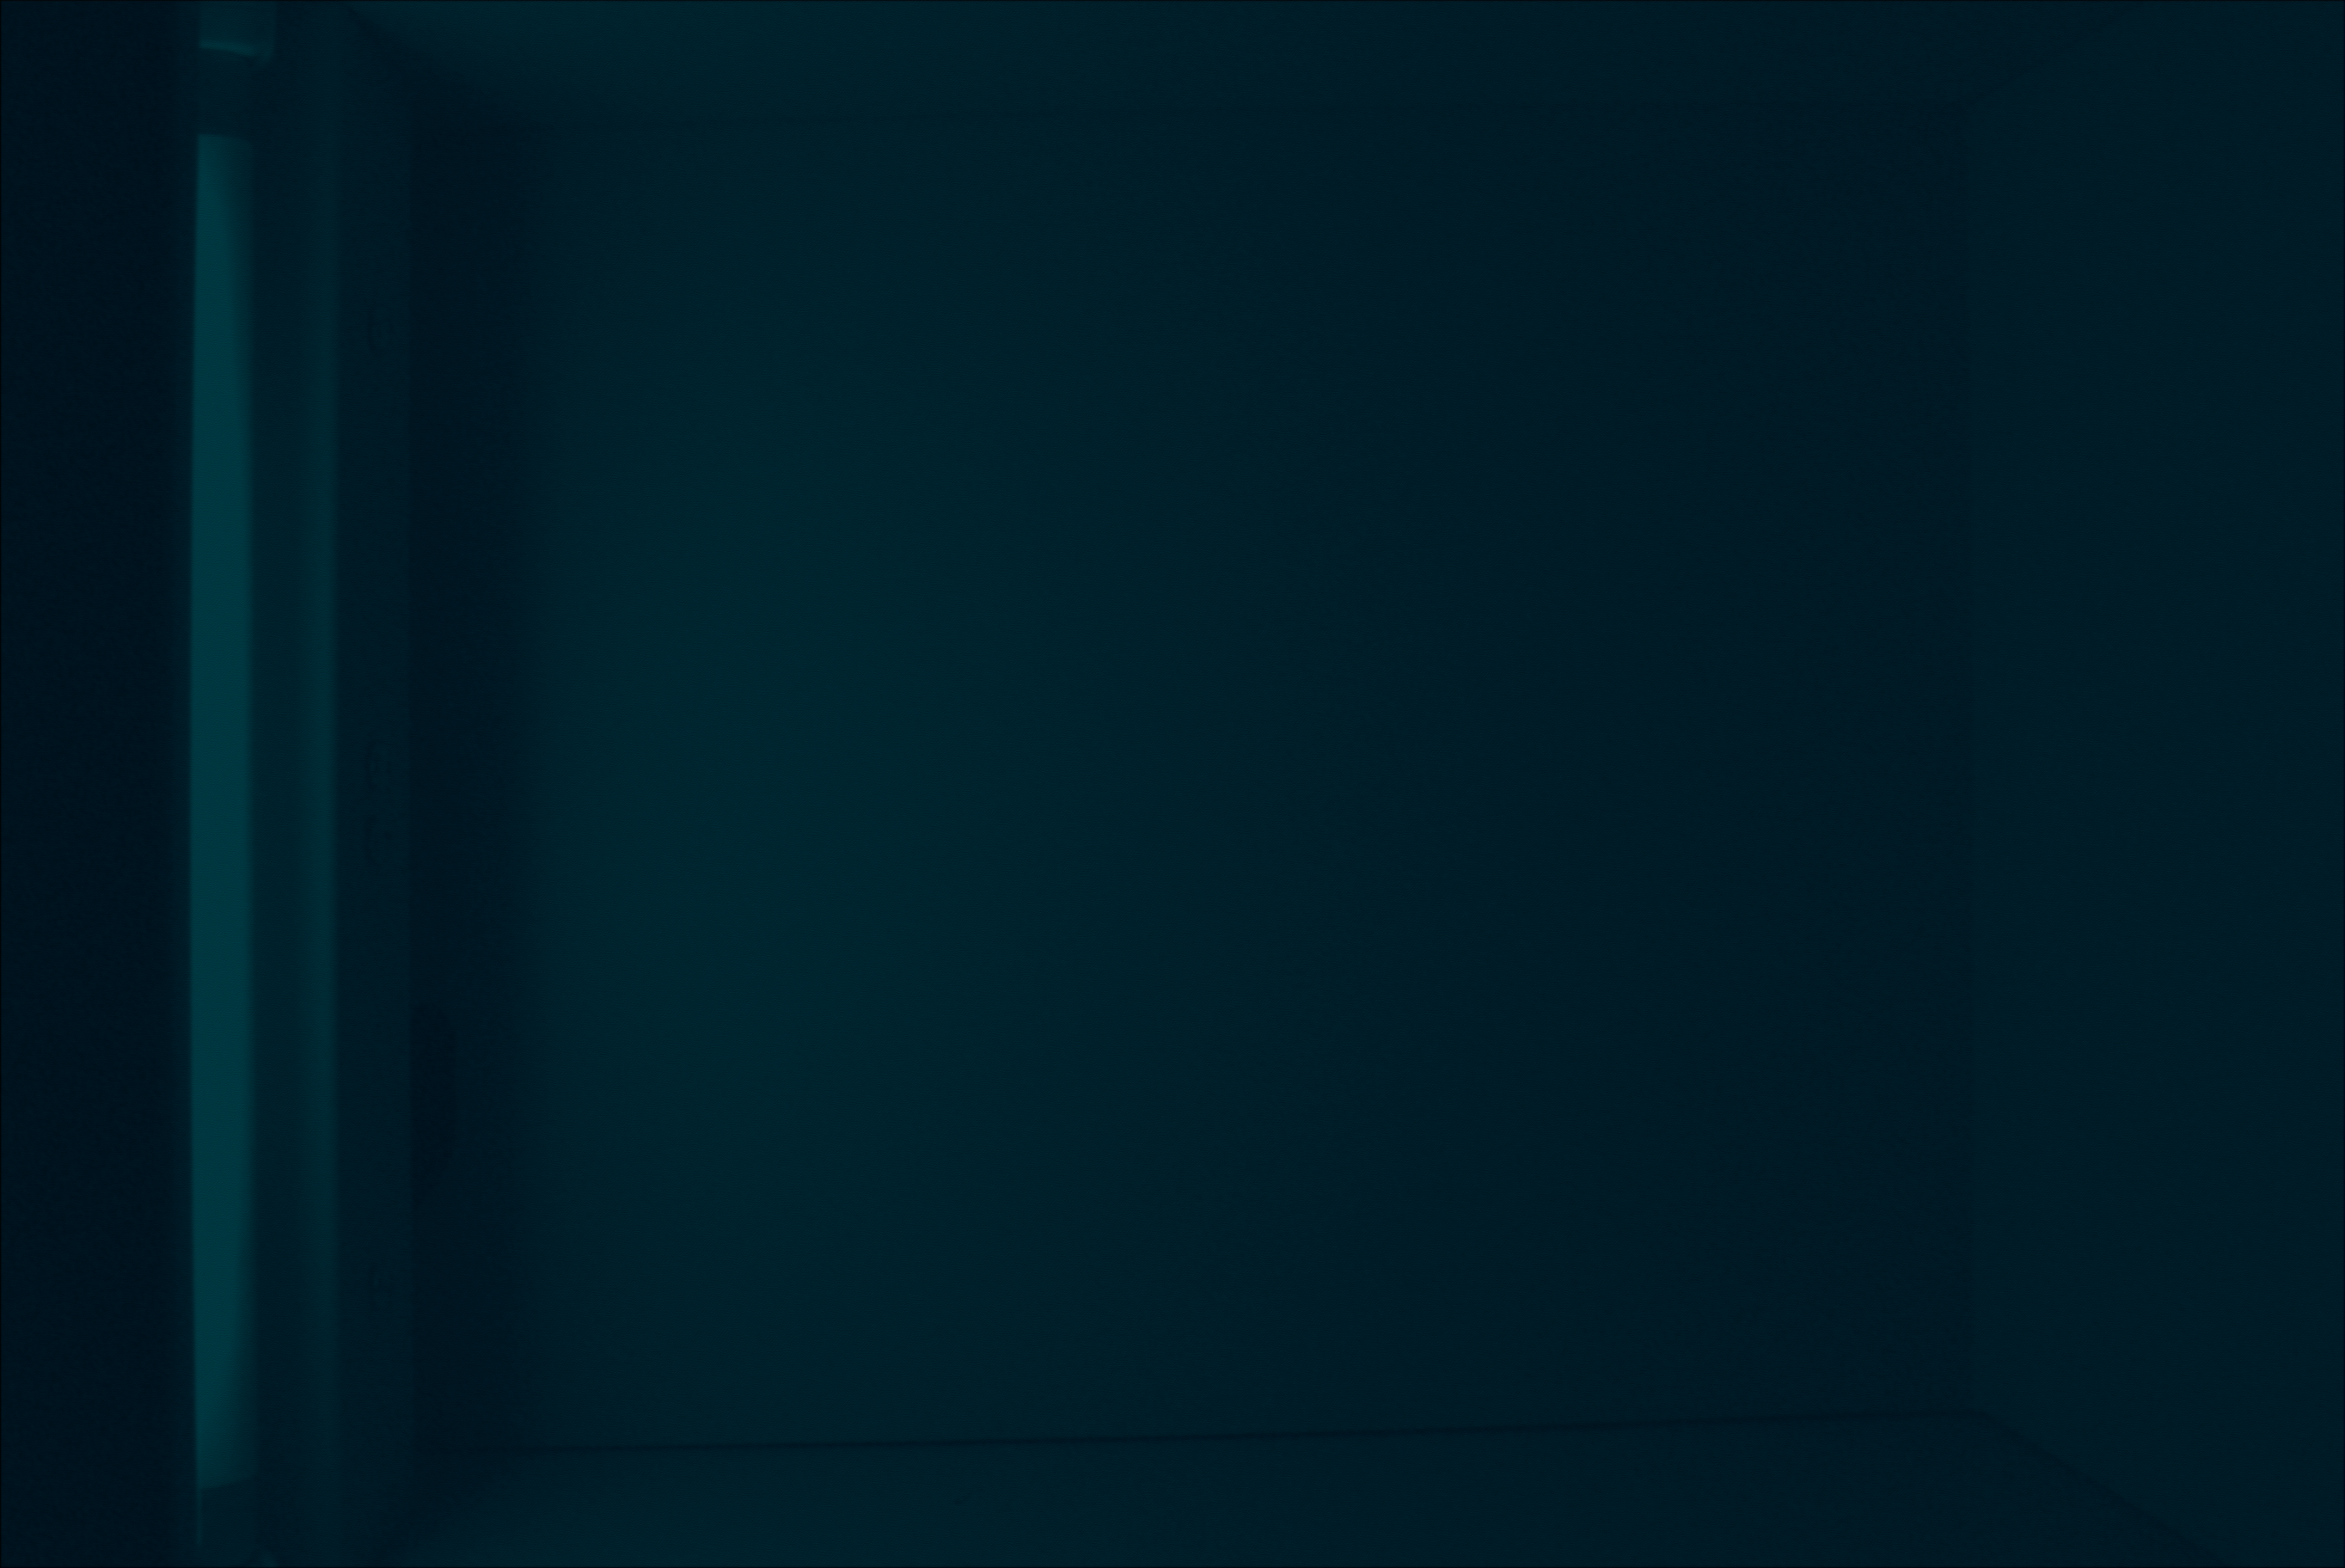
\includegraphics[width=\linewidth]{figures/tv-rel-single.png}
        \caption{TV-Rel \\ noise, no resize \\ LPIPS: \textbf{0.27} \\ SSIM: 0.27}
    \end{subfigure}
    \hfill
    \begin{subfigure}[t]{.19\textwidth}
        \centering
        \includegraphics[width=\linewidth]{figures/digital-single.png}
        \caption{Baseline \\ \\ LPIPS: 0.36 \\ SSIM: 0.64}
      \end{subfigure}
  
    \caption{\textbf{Single Image Select Samples.} Outputs from select loss functions and configurations of noise and resizing. We see that the best performing model is MSE/VGG with resizing, which produces the best colour effect. We also see that LPIPS scores are inconsistent with SSIM and with perception as we can intuitively see that MSE-VGG and MSE are better predicitions than the baseline and TV-Rel.}

    \label{fig:single-image-samples}
\end{figure}

\begin{table}
    \centering
    \captionsetup{justification=centering}
    \caption{
        \textbf{Single Image Losses.} \\Results for each loss configuration with and without noise and no resizing.
    }
    \setlength{\tabcolsep}{0.3em}
    \begin{tabular}{l|cccc|cccc}
        \toprule
        \multicolumn{1}{c}{\textbf{Loss}}& \multicolumn{4}{c}{\textbf{Without Noise}} & \multicolumn{4}{c}{\textbf{With Noise}}\\
        \multicolumn{1}{c}{} & SSIM & PSNR & LPIPS & \multicolumn{1}{c}{PieAPP} & SSIM & PSNR & LPIPS & PieAPP \\
        \midrule
        Color/VGG/TV-Rel & \textbf{0.68} & 19.67 & 0.45 & \textbf{1.42} & 0.67 & 18.01 & 0.37 & \textbf{1.14} \\
        Color/VGG & \textbf{0.68} & \textbf{20.07} & 0.45 & 1.61 & \textbf{0.68} & 17.94 & 0.36 & 1.58 \\
        MSE/VGG & 0.66 & 18.26 & 0.48 & 2.53 & 0.67 & \textbf{19.79} & 0.34 & 2.05 \\
        MAE & 0.65 & 18.61 & 0.50 & 2.12 & \textbf{0.68} & 19.04 & 0.33 & 1.96 \\
        Color & 0.65 & 18.45 & 0.50 & 2.99 & 0.63 & 15.66 & 0.43 & 2.50 \\
        MSE & 0.65 & 18.29 & 0.50 & 2.42 & 0.67 & 19.26 & 0.32 & 1.89 \\
        Baseline & 0.64 & 16.97 & \textbf{0.36} & 3.79 & 0.64 & 16.97 & 0.36 & 3.79 \\
        \midrule
        TV-Rel & 0.17 & 9.84 & 0.60 & 4.84 & 0.27 & 11.11 & \textbf{0.27} & 2.20 \\
        VGG & 0.16 & 9.10 & 0.62 & 4.50 & 0.06 & 8.71 & 0.64 & 5.11 \\
        \bottomrule
    \end{tabular}
    
    \label{tab:single-image-losses}
\end{table}


The addition of noise has mixed effects. The perceptual metrics significantly reward the addition of noise in almost all cases. SSIM and PSNR react differently depending on the loss: pixel-wise MSE/MAE scores increase slightly, whereas Color loss scores decrease. This can be interpreted as Color loss allowing more noise through the model which is penalised by metrics sensitive to incorrect random noise such as PSNR, where MAE/MSE will even out this noise to be closer to the ground truth, on average. All of this implies that the perceptual metrics better capture the output of noise by the model. Comparisons of outputs from the models with and without noise channels can be seen in Figure \ref{fig:single-image-noise-no-noise}.

\begin{figure}

    \begin{subfigure}[t]{.24\textwidth}
        \centering
        \includegraphics[width=\linewidth]{figures/color-vgg-tv-rel-noise-patch-single.png}
        
      \end{subfigure}
    \hfill
    \begin{subfigure}[t]{.24\textwidth}
        \centering
        \includegraphics[width=\linewidth]{figures/mse-vgg-noise-no-resize-patch-single.png}
    \end{subfigure}
    \hfill
    \begin{subfigure}[t]{.24\textwidth}
        \centering
        \includegraphics[width=\linewidth]{figures/mse-noise-no-resize-patch-single.png}
    \end{subfigure}
    \hfill
    \begin{subfigure}[t]{.24\textwidth}
        \centering
        \includegraphics[width=\linewidth]{figures/film-patch-single.png}
      \end{subfigure}


    \begin{subfigure}[t]{.24\textwidth}
        \centering
        \includegraphics[width=\linewidth]{figures/color-vgg-tv-rel-no-noise-patch-single.png}
        \captionsetup{justification=centering}
        \caption{Color/VGG/TV-Rel}
      \end{subfigure}
        \hfill
    \begin{subfigure}[t]{.24\textwidth}
        \centering
        \includegraphics[width=\linewidth]{figures/mse-vgg-no-noise-no-resize-patch-single.png}
        \caption{\\MSE/VGG}
      \end{subfigure}
    \hfill
    \begin{subfigure}[t]{.24\textwidth}
        \centering
        \includegraphics[width=\linewidth]{figures/mse-no-noise-no-resize-patch-single.png}
        \caption{\\MSE}
    \end{subfigure}
    \hfill
    \begin{subfigure}[t]{.24\textwidth}
        \centering
        \includegraphics[width=\linewidth]{figures/digital-patch-single.png}
        \captionsetup{justification=centering}
        \caption{Film (Above) \\ Digital (Below)}
      \end{subfigure}
   
      \centering

    \caption{\textbf{Single Image Noise Comparison.} Outputs from select models without noise (above) and with noise (below), no resizing. We see that when we feed noise into the model, the model learns to produce some variation, especially when the loss contains a feature-based metric like VGG. However, the grain is far from the desired effect.}
    \label{fig:single-image-noise-no-noise}
\end{figure}

We also experiment with resizing cropped patches during training. This is done by taking a crop at a random scale from the image and resizing it to the patch size, $ 256 \times 256$. The results are in Table \ref{tab:single-image-resize}. We show results for only MSE and MSE/VGG as a representative example of how both pixel-wise and combined losses perform. We also experimented with a combination of noise and resizing but found that both performed better alone.  We find that we reach peak SSIM and PSNR scores when resizing the cropped patches, and perceptual metrics also improve across the board.

We hypothesise that while resizing loses high-resolution information on grain and noise patterns, the model sees a greater variety of areas of the image in a single patch and so may capture the color transformation better which is rewarded by every metric. With the MSE/VGG loss, this colour transformation is a nearly perfect overfit as the outputs in \ref{fig:single-image-resize} show. Furthermore, some grain is still produced when we feed noise into the model despite the resizing operation potentially removing grain, as can be seen in Figure \ref{fig:single-image-resize-noise}.


\begin{figure}[ht]
    \centering

    \begin{subfigure}[b]{0.49\textwidth}
        \centering
        \includegraphics[width=0.49\textwidth]{figures/mse-vgg-no-noise-no-resize-single.png}
        \includegraphics[width=0.49\textwidth]{figures/mse-vgg-no-noise-resize-single.png}
        \captionsetup{justification=centering}
        \caption{MSE/VGG, no noise \\ no resize (left) and with resizing (right).}
    \end{subfigure}
    \hfill
    \begin{subfigure}[b]{0.49\textwidth}
        \centering
        \includegraphics[width=0.49\textwidth]{figures/mse-no-noise-no-resize-single.png}
        \includegraphics[width=0.49\textwidth]{figures/mse-no-noise-resize-single.png}
        \captionsetup{justification=centering}
        \caption{MSE, no noise \\ no resize (left) and with resizing (right).} 
    \end{subfigure}
    \caption{\textbf{Single Image Resizing.} Outputs from MSE and MSE/VGG with and without resizing, and then with resizing and with and without noise. We see that resizing improves the colour effect, but the grain effect is not as strong as in the single image experiments.}
    \label{fig:single-image-resize}
\end{figure}
\begin{figure}[ht]
    \begin{subfigure}[b]{0.49\textwidth}
        \centering
        \includegraphics[width=0.49\textwidth]{figures/mse-vgg-no-noise-resize-patch-single.png}
        \includegraphics[width=0.49\textwidth]{figures/mse-vgg-noise-resize-patch-single.png}
        \captionsetup{justification=centering}
        \caption{MSE/VGG patch with resizing \\ no noise (left) and with noise (right).} 
    \end{subfigure}
    \hfill
    \begin{subfigure}[b]{0.49\textwidth}
        \centering
        \includegraphics[width=0.49\textwidth]{figures/mse-no-noise-resize-patch-single.png}
        \includegraphics[width=0.49\textwidth]{figures/mse-noise-resize-patch-single.png}
        \captionsetup{justification=centering}
        \caption{MSE patch with resizing \\ no noise (left) and with noise (right).}
    \end{subfigure}

    \caption{\textbf{Single Image Resizing with Noise.} Outputs from MSE and MSE/VGG with and without noise and resizing. We see that similar grain is still produced even through resizing.}
    \label{fig:single-image-resize-noise}
\end{figure}

\begin{table}
    \centering
    \captionsetup{justification=centering}
    \setlength{\tabcolsep}{0.5em}
    \caption{
        \textbf{Single Image Resizing.} \\ Effect of resizing the cropped patches on select losses (no noise).
    }
    \begin{tabular}{lccccc}
        \toprule
        \multicolumn{1}{c}{Loss}& \multicolumn{1}{c}{Resize}&  SSIM & PSNR & LPIPS & PieAPP\\
        \midrule
        MSE/VGG & Yes & \textbf{0.71} & \textbf{23.19} & \textbf{0.35} & \textbf{1.62} \\
        MSE/VGG & No & 0.66 & 18.26 & 0.48 & 2.53 \\
        \midrule
        MSE & Yes & \textbf{0.67} & \textbf{20.03} & \textbf{0.47} & \textbf{1.77} \\
        MSE & No & 0.65 & 18.29 & 0.50 & 2.42 \\

        \bottomrule
    \end{tabular}
    
    \label{tab:single-image-resize}
\end{table}


\subsection{Full Dataset Results}

We select the best performing losses and settings from the single image experiments and evaluate them on the full dataset, with results in Table \ref{tab:full-data-results}.

\begin{table}
    \centering
    \captionsetup{justification=centering}
    \caption{\textbf{Full Dataset Results.} \\ Comparison of best performing losses and configurations on the full dataset.}
    \setlength{\tabcolsep}{0.3em}
    \begin{tabular}{lcccccc}
        \toprule
        Loss & Noise & Resize & SSIM & PSNR & LPIPS & PieAPP \\
        \midrule
        Baseline & - & - & \textbf{0.64} & 21.68 & \textbf{0.26} & 1.96 \\
        MSE/VGG & Yes & Yes & \textbf{0.64} & \textbf{22.87} & 0.27 & \textbf{1.90} \\
        MSE & No & Yes & 0.63 & 22.20 & 0.35 & 2.31 \\
        MAE & No & No & 0.59 & 19.68 & 0.48 & 3.38 \\
        Color/VGG/TV-Rel & Yes & No & 0.59 & 21.42 & 0.41 & 3.07 \\
        MSE/VGG/TV-Rel & Yes & No & 0.58 & 20.43 & 0.46 & 3.54 \\
        \bottomrule
    \end{tabular}
    \label{tab:full-data-results}
\end{table}

We selected models in terms of high scoring metrics and qualitative evaluation of color and grain production. This leaves us with some models that should produce the best colour: MSE/VGG and MSE with resizing, and other models that should produce the best grain: Color/VGG/TV-Rel, MSE/VGG/TV-Rel with a noise input channel. We find that the best performing model is MSE/VGG with resizing which produces the best metrics across the board. A notable difference compared to the single image results is that our methods now almost never outperform the baseline despite training on the same number of patches per image. This is likely due to the increased complexity of the full dataset, which contains a wider variety of film effects and lighting conditions. The only exception is MSE/VGG which is on par with the baseline. A sample of results can be seen in Figure \ref{fig:full-data-results}.


\begin{figure}

    % Chess
    \begin{subfigure}[t]{.24\textwidth}
        \centering
        \includegraphics[width=\linewidth]{figures/digital-chess.png}
      \end{subfigure}
    \hfill
    \begin{subfigure}[t]{.24\textwidth}
        \centering
        \includegraphics[width=\linewidth]{figures/film-chess.png}
      \end{subfigure}
    \hfill
    \begin{subfigure}[t]{.24\textwidth}
        \centering
        \includegraphics[width=\linewidth]{figures/mse-vgg-noise-resize-chess.png}
      \end{subfigure}
    \hfill
    \begin{subfigure}[t]{.24\textwidth}
      \centering
      \includegraphics[width=\linewidth]{figures/color-vgg-tv-relative-chess.png}
    \end{subfigure}

    % Swisstech
    \begin{subfigure}[t]{.24\textwidth}
        \centering
        \includegraphics[width=\linewidth]{figures/digital-swisstech.png}
      \end{subfigure}
    \hfill
    \begin{subfigure}[t]{.24\textwidth}
        \centering
        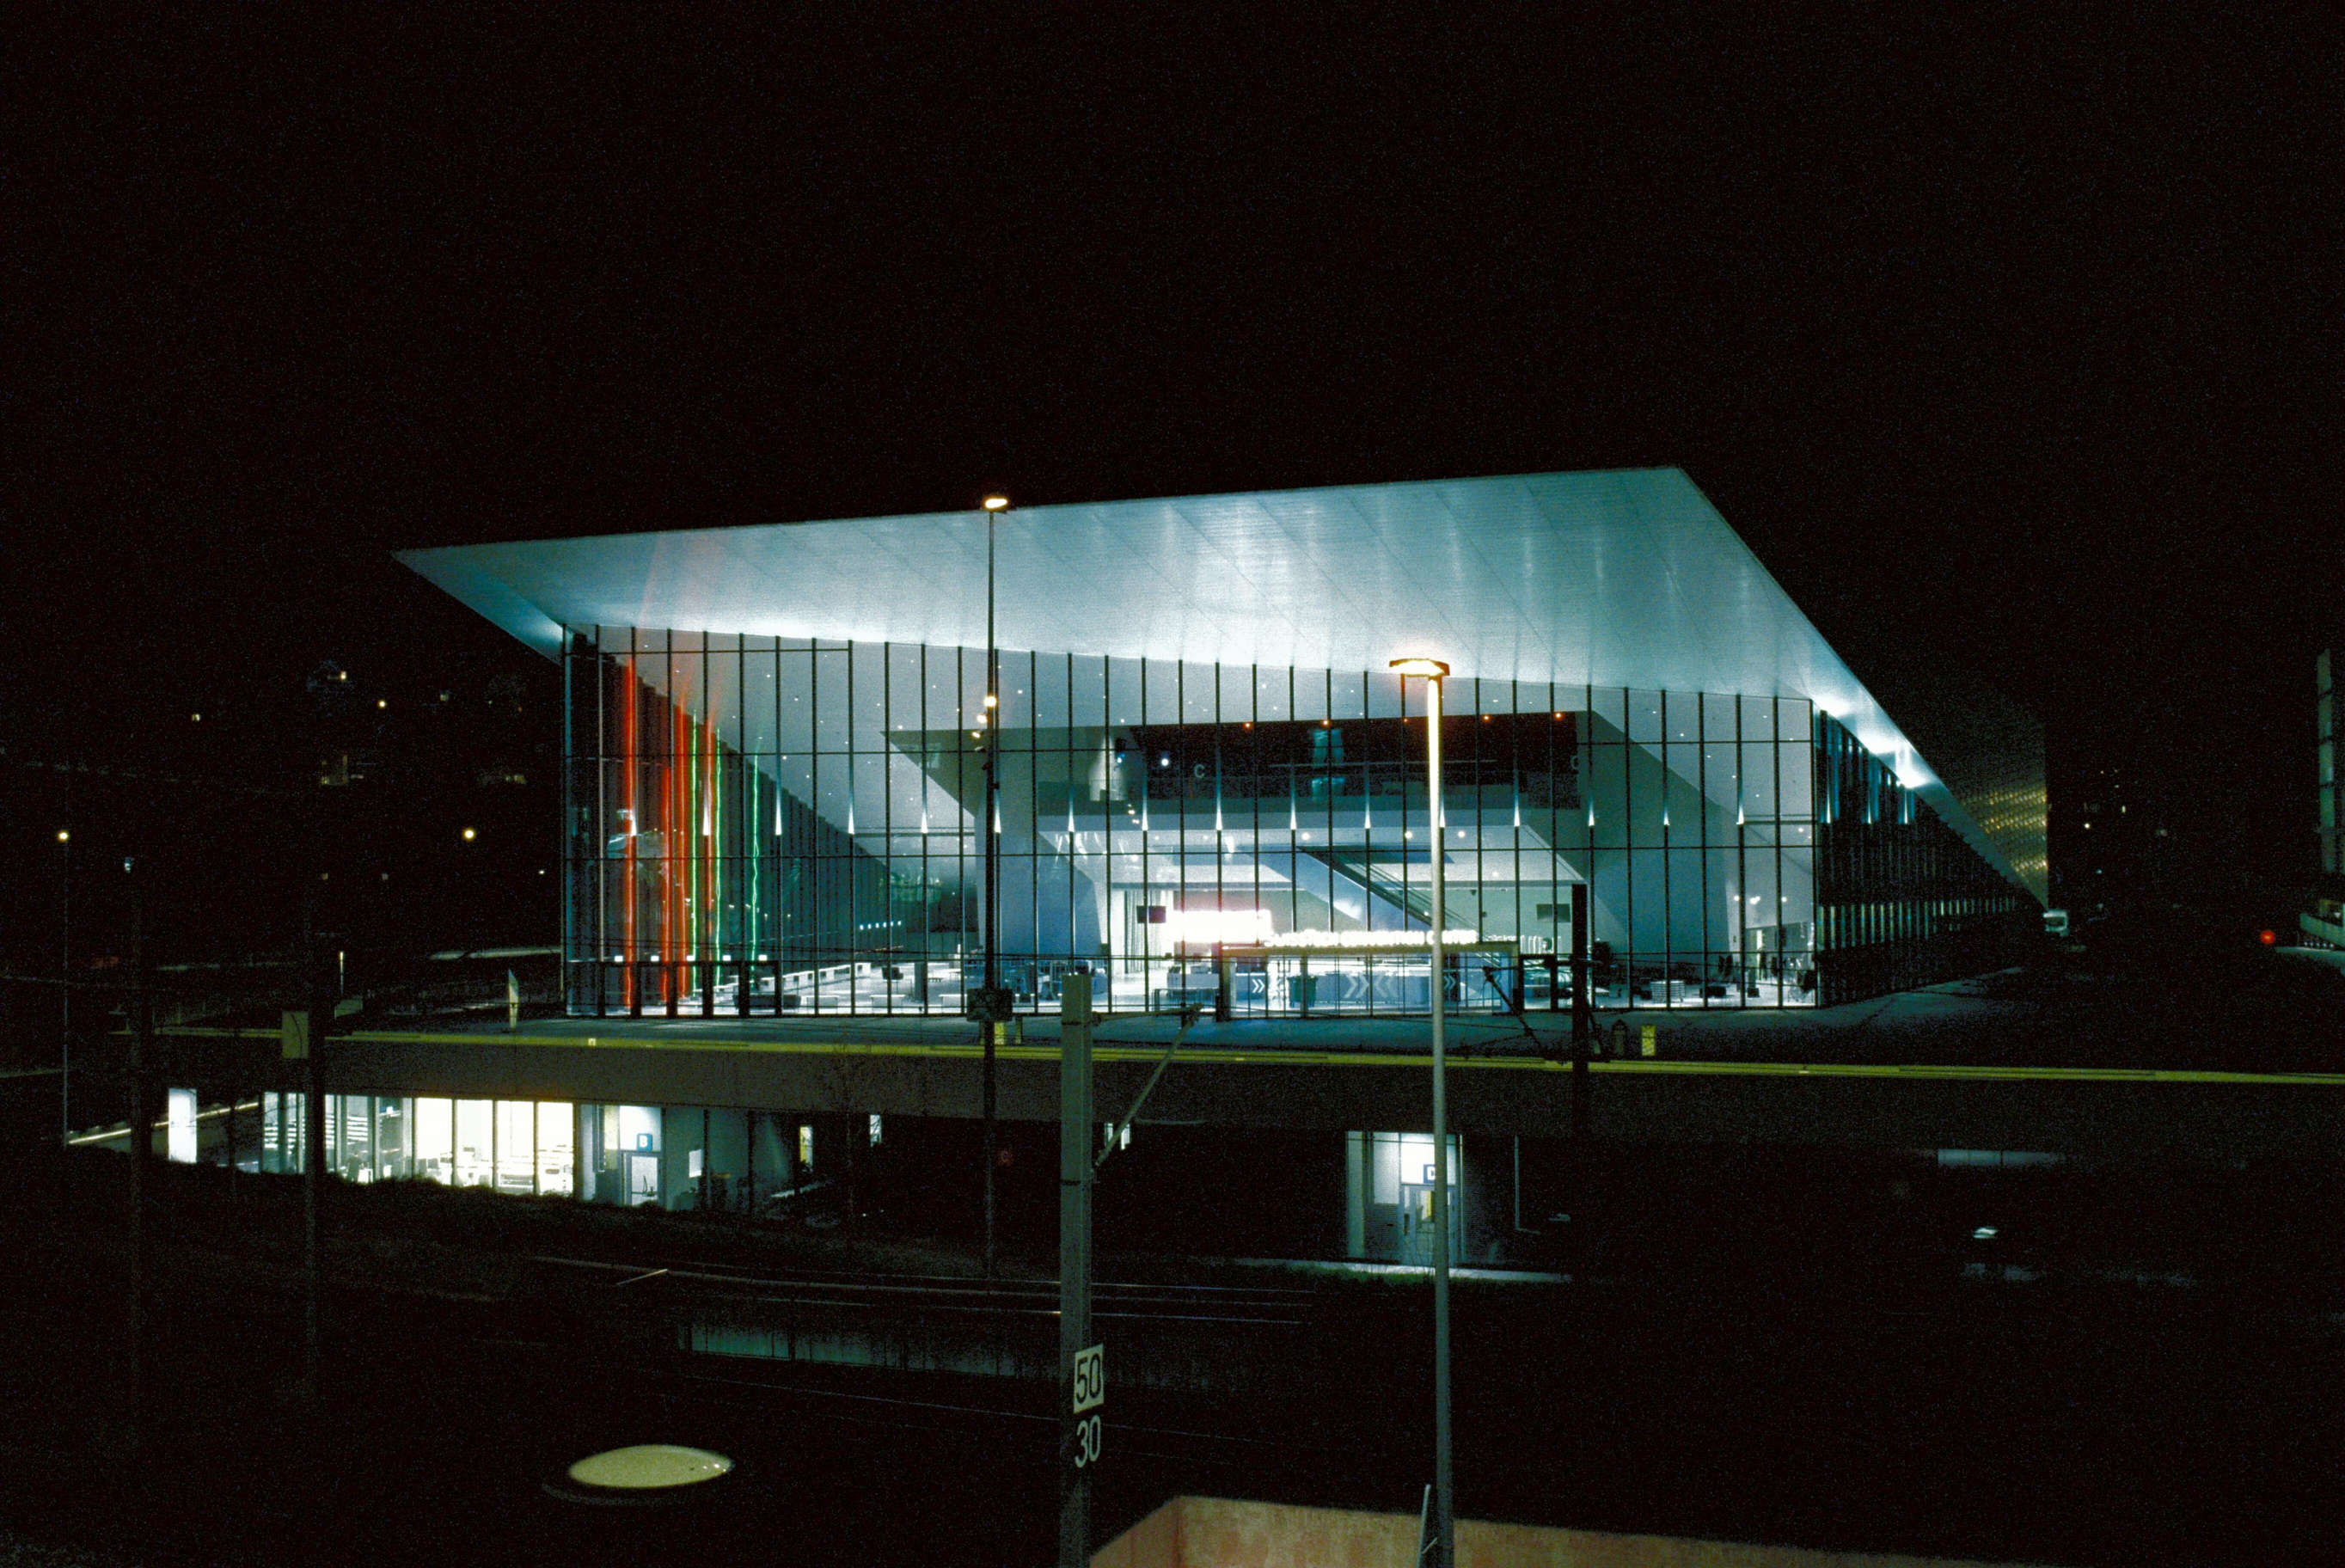
\includegraphics[width=\linewidth]{figures/film-swisstech.png}
      \end{subfigure}
    \hfill
    \begin{subfigure}[t]{.24\textwidth}
        \centering
        \includegraphics[width=\linewidth]{figures/mse-vgg-noise-resize-swisstech.png}
      \end{subfigure}
    \hfill
    \begin{subfigure}[t]{.24\textwidth}
      \centering
      \includegraphics[width=\linewidth]{figures/color-vgg-tv-relative-swisstech.png}
    \end{subfigure}


    % Castle
    \begin{subfigure}[t]{.24\textwidth}
        \centering
        \includegraphics[width=\linewidth]{figures/digital-castle.png}
        \captionsetup{justification=centering}
        \caption{\\Digital}
      \end{subfigure}
    \hfill
    \begin{subfigure}[t]{.24\textwidth}
        \centering
        \includegraphics[width=\linewidth]{figures/film-castle.png}
        \captionsetup{justification=centering}
        \caption{\\Film}
      \end{subfigure}
    \hfill
    \begin{subfigure}[t]{.24\textwidth}
        \centering
        \includegraphics[width=\linewidth]{figures/mse-vgg-noise-resize-castle.png}
        \captionsetup{justification=centering}
        \caption{\\MSE/VGG}
      \end{subfigure}
    \hfill
    \begin{subfigure}[t]{.24\textwidth}
      \centering
      \includegraphics[width=\linewidth]{figures/color-vgg-tv-relative-castle.png}
      \captionsetup{justification=centering}
        \caption{\\Color/VGG/TV-Rel}
    \end{subfigure}

    \caption{\textbf{Full Dataset Select Samples.} Outputs from select models on the full dataset. We see that the best performing model is MSE/VGG with resizing, which produces the best colour effect. We also see that the grain effect is not as strong as in the single image experiments.}
    \label{fig:full-data-results}
\end{figure}

We continue experimenting with the presence of resizing and noise using MSE and MSE/VGG, with results found in Table \ref{tab:full-data-resize-noise}. Results indicate that once again resizing improves results, but the addition of noise has a less clear effect. The overall best performing model is MSE/VGG with resizing. Noise has little effect. However, the qualitative results tell a different story. In Figure \ref{fig:full-data-grain} we see that the model with noise produces a more visually pleasing result, with a more uniform grain effect. This is not captured by the metrics, which are more sensitive to the colour effect.

\begin{table}
    \centering
    \captionsetup{justification=centering}
    \caption{\textbf{Full Dataset Noise and Resizing.} \\ Comparison of MSE and MSE/VGG with and without noise and resizing.}
    \setlength{\tabcolsep}{0.3em}
    \begin{tabular}{lcccccc}
        \toprule
        Loss & Noise & Resize & SSIM & PSNR & LPIPS & PieAPP \\
        \midrule
        MSE/VGG & Yes & Yes & \textbf{0.64} & \textbf{22.87} & \textbf{0.27} & 1.90 \\
        MSE/VGG & No & Yes & 0.63 & 22.85 & \textbf{0.27} & \textbf{1.84} \\
        MSE/VGG & No & No & 0.58 & 20.47 & 0.50 & 3.67 \\
        \midrule
        MSE & No & Yes & \textbf{0.63} & \textbf{22.20} & \textbf{0.35} & \textbf{2.31} \\
        MSE & Yes & Yes & 0.59 & 20.87 & 0.40 & 3.29 \\
        MSE & No & No & 0.58 & 20.47 & 0.50 & 3.67 \\
        \bottomrule
    \end{tabular}
    \label{tab:full-data-resize-noise}
\end{table}

\begin{figure}
    \begin{subfigure}[t]{.19\textwidth}
        \centering
        \includegraphics[width=\linewidth]{figures/digital-sky.png}
        \captionsetup{justification=centering}
        \caption{Digital}
      \end{subfigure}
    \hfill
    \begin{subfigure}[t]{.19\textwidth}
        \centering
        \includegraphics[width=\linewidth]{figures/film-sky.png}
        \captionsetup{justification=centering}
        \caption{Film}
      \end{subfigure}
    \hfill
    \begin{subfigure}[t]{.19\textwidth}
        \centering
        \includegraphics[width=\linewidth]{figures/mse-vgg-noise-resize-sky.png}
        \captionsetup{justification=centering}
        \caption{MSE/VGG}
      \end{subfigure}
    \hfill
    \begin{subfigure}[t]{.19\textwidth}
        \centering
        \includegraphics[width=\linewidth]{figures/mse-vgg-tev-rel-sky.png}
        \captionsetup{justification=centering}
        \caption{MSE/VGG/TV-Rel}
      \end{subfigure}
      \begin{subfigure}[t]{.19\textwidth}
        \centering
        \includegraphics[width=\linewidth]{figures/color-vgg-tv-rel-sky.png}
        \captionsetup{justification=centering}
        \caption{Color/VGG/TV-Rel}
      \end{subfigure}
    \caption{\textbf{Full Dataset Grain Comparison.} Predictions for a patch of sky from select loss functions, all with noise. Similarly to the single image experiments, the models with losses that target some noise produce a more visually pleasing result. The best visual result is produced by Color/VGG/TV-Rel although this is still far from the true grain texture.}
    \label{fig:full-data-grain}
\end{figure}

% Comparison to DSLR results

Comparing results with the related task of enhancement of mobile phone images in \cite{dslr-quality} indicates that our models have a much lower SSIM, but comparable PSNR. They achieve peak SSIM of 0.94 where we observe a peak SSIM of 0.64, whereas peak PSNR is 21.81 and 22.87 respectively. This could be due to a large range of factors such as the the quality and uniformity of the DSLR images, the difference in model architecures or the difference in losses. However, perhaps the biggest reason is the greater complexity of the film effect.

% Summary

In summary, we find that the best performing model is MSE/VGG with resizing, which produces the best metrics across the board, produces the best colour effect and often the most visually pleasing result too. The addition of noise has mixed effects but tends to help in noise production, and resizing the cropped patches during training significantly improves the learned colour transformation. The perceptual metrics better capture the output of noise by the model, and resizing allows the model to see a greater variety of areas of the image in a single patch. However, the full dataset is more complex and the models do not outperform the baseline as they did in the single image experiments. Our best model learns a good colour mapping, but the grain effect is not as strong as in the single image experiments, nor is it exactly the kind of grain observed.


% --------------------------- %

% Example 1: Exclude resized crop experiments
% \begin{table}
%     \centering
%     \caption{
%         \textbf{Full Data.}
%     }
%     \begin{tabular}{lc|cccc}
%         \toprule
%         \multicolumn{2}{c}{\textbf{Configuration}}& \multicolumn{4}{c}{\textbf{Evaluation}} \\
%         Loss & Noise & SSIM & PSNR & LPIPS & PieAPP \\
%         \midrule
%         \textbf{Baseline} & - & \textbf{0.64} {\tiny $\pm 0.09$} & \textbf{21.68} {\tiny $\pm 2.02$} & \textbf{0.26} {\tiny$\pm 0.07$} & \textbf{1.96} {\tiny $\pm 0.83$} \\
%         MAE & No & 0.59 {\tiny $\pm 0.09$} & 19.68 {\tiny $\pm 2.28$} & 0.48 {\tiny$\pm 0.08$} & 3.38 {\tiny $\pm 0.67$} \\
%         Color + VGG + TV-Rel & Yes & 0.59 {\tiny $\pm 0.11$} & 21.42 {\tiny $\pm 2.13$} & 0.41 {\tiny$\pm 0.06$} & 3.07 {\tiny $\pm 0.78$} \\
%         MSE & No & 0.58 {\tiny $\pm 0.10$} & 20.47 {\tiny $\pm 2.16$} & 0.50 {\tiny$\pm 0.08$} & 3.67 {\tiny $\pm 0.88$} \\
%         MSE + VGG & No & 0.58 {\tiny $\pm 0.10$} & 20.47 {\tiny $\pm 2.16$} & 0.50 {\tiny$\pm 0.08$} & 3.67 {\tiny $\pm 0.88$} \\
%         MSE + VGG + TV-Rel & Yes & 0.58 {\tiny $\pm 0.11$} & 20.43 {\tiny $\pm 2.29$} & 0.46 {\tiny$\pm 0.08$} & 3.54 {\tiny $\pm 0.76$} \\
%         \hline
%         \bottomrule
%     \end{tabular}
%     \label(tab:full-data-results)
% \end{table}
\section{Conclusion}
\label{sec:conclusion}

% Guidelines:
% - A short conclusion where you summarize what you have essentially done in your project, possible extensions or future work, as well as limitations.

%  Conclusion

In this work, we have explored the use of convolution neural networks in modeling the effect given by Cinestill800T film. We focused on the use of different loss functions as well as the addition of a noise channel to the input, and the use of random scales of patches during training. We find that a combination of MSE/VGG gives the best colour production which is significantly helped by resizing, and that the addition of a noise channel and another loss such as TV-Rel produces some grain.

Our contributions include the creation of a dataset of paired images taken with a film and digital camera, and all of our code in Pytorch, the details of which can be found in Section \ref{sec:code-documentation} in the appendix.

% Limitations & Future Work

Our results are severely limited by the small size and great variety of our dataset, meaning that the model must learn a complex function with relatively little training data. This is evidenced by the lack of sign of halation ever being produced by our models, as they were simply not trained on enough patches containing halation. We also restricted ourselves to a pure deep learning approach, and did not explore the use of statistical models for film grain, halation, and colour hue.



\section{Further Work}
\label{sec:further-work}

While we tried many combinations of hyperpamaters, we did not rigorously explore all options. Further work could systematically investigate the effect of kernel size, model size, patch size or the weightings for each loss function when combined. The dataset could be also narrowed focused to include only scenes of a similar nature to give the model an easier function to learn. This could be taken to the extreme for halation, where only patches containing some halation could be fed to the model. A natural extension would be to condition the model on features of the image such as dynamic range. 

For grain production, an implicitly defined texture loss that more precisely captures the grain seen in films could be added, such as GCLM \cite{glcm} or notably an adversarial loss as in \cite{dslr-quality}. Avenues we only briefly explored could be tested in more depth. This includes the paired auto-encoder architecture from \cite{raw-to-raw} and the contextual bilateral loss from \cite{zoom-to-learn}, both contained in our code. Lastly, the model could be combined with a non-ML approach to see if a hybrid model can produce better results.

% References
\newpage
\bibliographystyle{splncs04}
\bibliography{main}

% Appendix
\newpage
\section{Appendix}
\label{sec:appendix}

% Guidelines
% - No page limits
% - Provide documentation for all of your codes. This will help the grading of your submitted codes, the clearer things are the easier it will be to understand your codes, to test them and to grade you fairly. 
% - If you have any proofs or any notes, you can also add them to the appendix.

\subsection{Code Documentation}
\label{sec:code-documentation}

The code for this project is available at \url{https://github.com/mikasenghaas/sillystill/tree/main}. The code is written in Python and uses \href{https://pytorch.org/}{PyTorch}, \href{https://lightning.ai/docs/pytorch/stable/}{Lightning} and \href{https://hydra.cc/}{Hydra} for configuration. The code is structured as follows:

\begin{itemize}
    \item \texttt{/src} contains the main code for the project, including the data processing, models, losses and training scripts.
        \begin{itemize}
            \item \texttt{/data} contains all datasets and Lightning datamodules. 
            \item \texttt{/models} contains the PyTorch model classes and loss functions.
            \item \texttt{/eval} contains wrapper classes for evaluation metrics.
            \item \texttt{/utils} contains a variety of utility functions.
            \item \texttt{train.py} is the main training script.
            \item \texttt{dev.py} is a developer script for testing code without using Lightning or Hydra.
            \item \texttt{preprocess.py} is a script for preprocessing the dataset.
            \item \texttt{evaluate.py} is an evaluation script.
            \item \texttt{unsplash.py} is a script for downloading images from Unsplash.
        \end{itemize}
    \item \texttt{/data} contains our dataset
    \item \texttt{/configs} contains the Hydra configuration files for the experiments.
    \item \texttt{/notebooks} contains Jupyter notebooks for investigating the data processing, losses, models and evaluation.
    \item \texttt{/report} contains the Latex files for the report.
\end{itemize}

In order to train a model, the \texttt{src/train.py} script can be run with the desired configuration. You can specify a hydra configuration with flags or by editing the configuration files. The two experiments in this report can be run with the following commands:

\begin{verbatim}
python src/train.py experiment=single-image logger=none
python src/train.py experiment=full-data logger=none
\end{verbatim}

To edit the loss functions or other parameters, you can edit the configuration file \texttt{configs/experiment/single-image.yaml}. The model will be trained, and inference will be run automatically, with results logged locally. If you want to log  to weights and biases, you can remove the logger flag.

\newpage
\subsection{All Results}
\label{sec:all-results}

\begin{table}[ht]
    \scriptsize
    \centering
    \caption{
        \textbf{Single Image.} All Results}
    \begin{tabular}{lcc|cccc}
        \toprule
        \multicolumn{3}{c}{\textbf{Configuration}}& \multicolumn{4}{c}{\textbf{Evaluation}} \\
        Loss & Noise & Resized & SSIM & PSNR & LPIPS & PieAPP \\
        \midrule
        MSE + VGG & No & Yes & \textbf{0.71} & \textbf{23.19} & 0.35 & 1.62 \\
        MAE & Yes & No & 0.68 & 19.04 & 0.33 & 1.96 \\
        Color + VGG + TV-Rel & No & No & 0.68 & 19.67 & 0.45 & 1.42 \\
        Color + VGG & No & No & 0.68 & 20.07 & 0.45 & 1.61 \\
        Color + VGG & Yes & No & 0.68 & 17.94 & 0.36 & 1.58 \\
        Color + VGG + TV-Rel & Yes & No  & 0.67 & 18.01 & 0.37 & \textbf{1.14} \\
        MSE & No & Yes & 0.67 & 20.03 & 0.47 & 1.77 \\
        MSE & Yes & No & 0.67 & 19.26 & 0.32 & 1.89 \\
        MSE + VGG & Yes & No & 0.67 & 19.79 & 0.34 & 2.05 \\
        MSE & Yes & Yes & 0.67 & 18.61 & 0.30 & 1.87 \\
        MSE + TV-Rel + VGG & Yes & No & 0.66 & 20.14 & 0.30 & 1.84 \\
        MSE + VGG & No & No & 0.66 & 18.26 & 0.48 & 2.53 \\
        MAE & No & No & 0.65 & 18.61 & 0.50 & 2.12 \\
        Color & No & No & 0.65 & 18.45 & 0.50 & 2.99 \\
        MSE & No & No & 0.65 & 18.29 & 0.50 & 2.42 \\
        \textbf{Baseline} & - & - & 0.64 & 16.97 & 0.36 & 3.79 \\
        \midrule
        Color & Yes & No & 0.63 & 15.66 & 0.43 & 2.50 \\
        TV-Rel & Yes & No & 0.27 & 11.11 & \textbf{0.27} & 2.20 \\
        TV-Rel & No & No & 0.17 & 9.84 & 0.60 & 4.84 \\
        VGG & No & No & 0.16 & 9.10 & 0.62 & 4.50 \\
        VGG & Yes & No & 0.06 & 8.71 & 0.64 & 5.11 \\
        \bottomrule
    \end{tabular}
    \label{tab:all-single-image-results}
\end{table}

\begin{table}[ht]
    \scriptsize
    \centering
    \setlength{\tabcolsep}{0.3em}
    \caption{\textbf{Full Dataset.} All results}
    \begin{tabular}{lcc|cccc}
        \toprule
        \multicolumn{3}{c}{\textbf{Configuration}} & \multicolumn{4}{c}{\textbf{Evaluation}} \\
        Loss & Resize & Noise & SSIM & PSNR & LPIPS & PieAPP \\
        \midrule
        \textbf{Baseline} & - & - & \textbf{0.64} & 21.68 & \textbf{0.26} & 1.96 \\
        \hline
        MSE + VGG & Yes & Yes & \textbf{0.64} & \textbf{22.87} & 0.27 & 1.90 \\
        MSE + VGG & Yes & No & 0.63 & 22.85 & 0.27 & \textbf{1.84} \\
        MSE & Yes & No & 0.63 & 22.20 & 0.35 & 2.31 \\
        MSE & Yes & No & 0.59 & 19.68 & 0.48 & 3.38 \\
        Color + VGG + TV-Rel & No & Yes & 0.59 & 21.42 & 0.41 & 3.07 \\
        MSE & No & No & 0.58 & 20.47 & 0.50 & 3.67 \\
        MSE + VGG & No & No & 0.58 & 20.47 & 0.50 & 3.67 \\
        MSE + VGG + TV-Rel & No & Yes & 0.58 & 20.43 & 0.46 & 3.54 \\
        \bottomrule
    \end{tabular}
    \label{tab:all-full-dataset-results}
\end{table}


% Example 1: Only show runs w/ resize
% \begin{table}
%     \centering
%     \caption{
%         \textbf{Single Image Results.} Only runs w/o resize
%     .}
%     \begin{tabular}{lc|cccc}
%         \toprule
%         \multicolumn{2}{c}{\textbf{Configuration}}& \multicolumn{4}{c}{\textbf{Evaluation}} \\
%         Loss & Noise & SSIM & PSNR & LPIPS & PieAPP \\
%         \midrule
%         MAE & Yes & 0.68 & 19.04 & 0.33 & 1.96 \\
%         Color + VGG + TV-Rel & No & 0.68 & 19.67 & 0.45 & 1.42 \\
%         Color + VGG & No & 0.68 & 20.07 & 0.45 & 1.61 \\
%         Color + VGG & Yes & 0.68 & 17.94 & 0.36 & 1.58 \\
%         Color + VGG + TV-Rel & Yes & 0.67 & 18.01 & 0.37 & \textbf{1.14} \\
%         MSE & Yes & 0.67 & 19.26 & 0.32 & 1.89 \\
%         MSE + TV-Rel + VGG & Yes & 0.66 & 20.14 & \textbf{0.30} & 1.84 \\
%         MSE + VGG & No & 0.66 & 18.26 & 0.48 & 2.53 \\
%         MAE & No & 0.65 & 18.61 & 0.50 & 2.12 \\
%         Color & No & 0.65 & 18.45 & 0.50 & 2.99 \\
%         MSE & No & 0.65 & 18.29 & 0.50 & 2.42 \\
%         \textbf{Baseline} & - & 0.64 & 16.97 & 0.36 & 3.79 \\
%         \hline
%         Color & Yes & 0.63 & 15.66 & 0.43 & 2.50 \\
%         TV-Rel & Yes & 0.27 & 11.11 & 0.27 & 2.20 \\
%         TV-Rel & No & 0.17 & 9.84 & 0.60 & 4.84 \\
%         VGG & No & 0.16 & 9.10 & 0.62 & 4.50 \\
%         VGG & Yes & 0.06 & 8.71 & 0.64 & 5.11 \\
%         TV-Abs & Yes & 0.00 & 4.96 & 0.60 & 19.05 \\
%         TV-Abs & No & 0.00 & 4.96 & 0.53 & 19.05 \\
%         \bottomrule
%     \end{tabular}
%     \label{tab:single-image-results}
% \end{table}

% Example 2: MSE w/ and w/o noise and resize
% Could be nice to show the influence of noise/ resize w/ MSE loss (only loss that has all combinations)
% \begin{table}
%     \centering
%     \caption{
%         \textbf{Single Image Results.} MSE Runs
%     .}
%     \begin{tabular}{lcc|cccc}
%         \toprule
%         \multicolumn{3}{c}{\textbf{Configuration}}& \multicolumn{4}{c}{\textbf{Evaluation}} \\
%         Loss & Noise & Resized & SSIM & PSNR & LPIPS & PieAPP \\
%         \midrule
%         MSE & No & Yes & \textbf{0.67} & \textbf{20.03} & 0.47 & \textbf{1.77} \\
%         MSE & Yes & No & 0.67 & 19.26 & 0.32 & 1.89 \\
%         MSE & Yes & Yes & 0.67 & 18.61 & \textbf{0.30} & 1.87 \\
%         MSE & No & No & 0.65 & 18.29 & 0.50 & 2.42 \\
%         \textbf{Baseline} & - & - & 0.64 & 16.97 & 0.36 & 3.79 \\
%         \bottomrule
%     \end{tabular}
% \end{table}



\end{document}
